\documentclass{article}

\usepackage{neurips_2026}

\usepackage[utf8]{inputenc}
\usepackage[T1]{fontenc}
\usepackage{hyperref}
\usepackage{url}
\usepackage{booktabs}
\usepackage{amsfonts}
\usepackage{amsmath}
\usepackage{nicefrac}
\usepackage{microtype}
\usepackage{xcolor}
\usepackage{graphicx}
\usepackage{array}
\usepackage{enumitem}
\usepackage{placeins}
\usepackage{tikz}
\usetikzlibrary{arrows.meta,positioning}

\newcommand{\method}[1]{\texttt{#1}}

\title{Q/R/M/C: A Stage-Decomposition Measurement Framework for Memory-Based Navigation}

%\author{%
%  Anonymous Authors \\
%  Anonymous Institution \\
%  Anonymous Address \\
%  \texttt{anonymous@anonymous.edu} \\
%}

\begin{document}

\maketitle

\begin{abstract}
\textbf{Setting.} Success-only metrics collapse qualitatively different memory-based navigation failures into a single scalar, hiding \emph{which stage} of the retrieval pipeline is responsible. This paper contributes an \emph{evaluation protocol}: the Q/R/M/C stage decomposition (\textbf{Q}uery formation, \textbf{R}etrieval satisfaction, target \textbf{M}aterialization, \textbf{C}ompletion after retrieval), operationalised so that the four conditional rates are computable directly from standard trajectory logs (Definition~1). The arithmetic is the chain rule, deliberately so --- just as decomposing accuracy into precision and recall added no mathematics but changed what the field could \emph{see}, the value here is identifiability from logs and what the decomposition reveals, not a theorem.
\textbf{Single-agent measurement.} On a 10-seed MiniGrid benchmark (FourRooms, LavaGapS7) and a BabyAI portability check, the framework localises bottlenecks: hazard recovery is retrieval-limited (oracle retrieval lifts success $0.39\to0.60$), goal-region rejoin is downstream-limited. Log inspection refines the attribution: candidate ranking is near-optimal ($96.9\%$) while candidate generation fails at 91\% of decision points --- a memory-accumulation, not a ranking, limit.
\textbf{Multi-agent measurement.} On a 35{,}640-run multi-agent sweep over four communication architectures (independent, shared-bus, central-aggregator, peer-broadcast at eight cadences $K{\in}\{1,2,4,8,16,32,48,64\}$, 40 seeds), the bottleneck-shift between the M and C links appears directly as a negative within-cadence correlation peaking at $K{=}4$ (Pearson $-0.61$); mean time-to-success has an interior minimum at $K{=}8$ (robust in location but shallow in margin --- not resolved from the adjacent fast cadences). Both slope signs (Empirical Claim~1) hold as moderate, cluster-robust effect sizes (Spearman $-0.53$ and $+0.43$ vs.\ $K$, 95\% CIs $[-0.59,-0.47]$ and $[+0.37,+0.50]$ over 81 configuration cells; Appendix~\ref{app:effect-sizes}). Non-claims (notably on the conditional product $\Phi$) are consolidated in one place (\S1, Scope and non-claims).
\textbf{Diagnostic use.} The same four rates also expose why learned policies with implicit communication can be competitive on success while collapsing Q/R/M/C observability: their communication vectors are never informatively empty and they lack an explicit target-lock interface. On two local LLM agents (qwen3:4b, llama3.1 on TextNav), the same logger localizes a completion-limited failure: under a tight step budget both agents form the query, retrieve, and lock the target ($Q^\star{=}R^\star{=}M^\star{=}1$) yet none complete ($C^\star{=}0$), so an otherwise opaque success collapse is resolved into a specific failing stage rather than a leaderboard number. Thus the contribution is a measurement protocol for making memory failures comparable across symbolic, learned, LLM, single-agent, and multi-agent systems.
\textbf{Scope.} The primary experiments are in grid-world substrates (MiniGrid, BabyAI, a custom $12{\times}10$ grid). The contribution is the diagnostic framework and its validation; a preliminary continuous-state check on VMAS reproduces both slope signs directionally (Appendix~\ref{app:vmas}), and a full continuous/3D validation with cluster-robust CIs (Habitat, ProcTHOR) is future work.
\end{abstract}

\section{Introduction}

\begin{figure}[t]
  \centering
  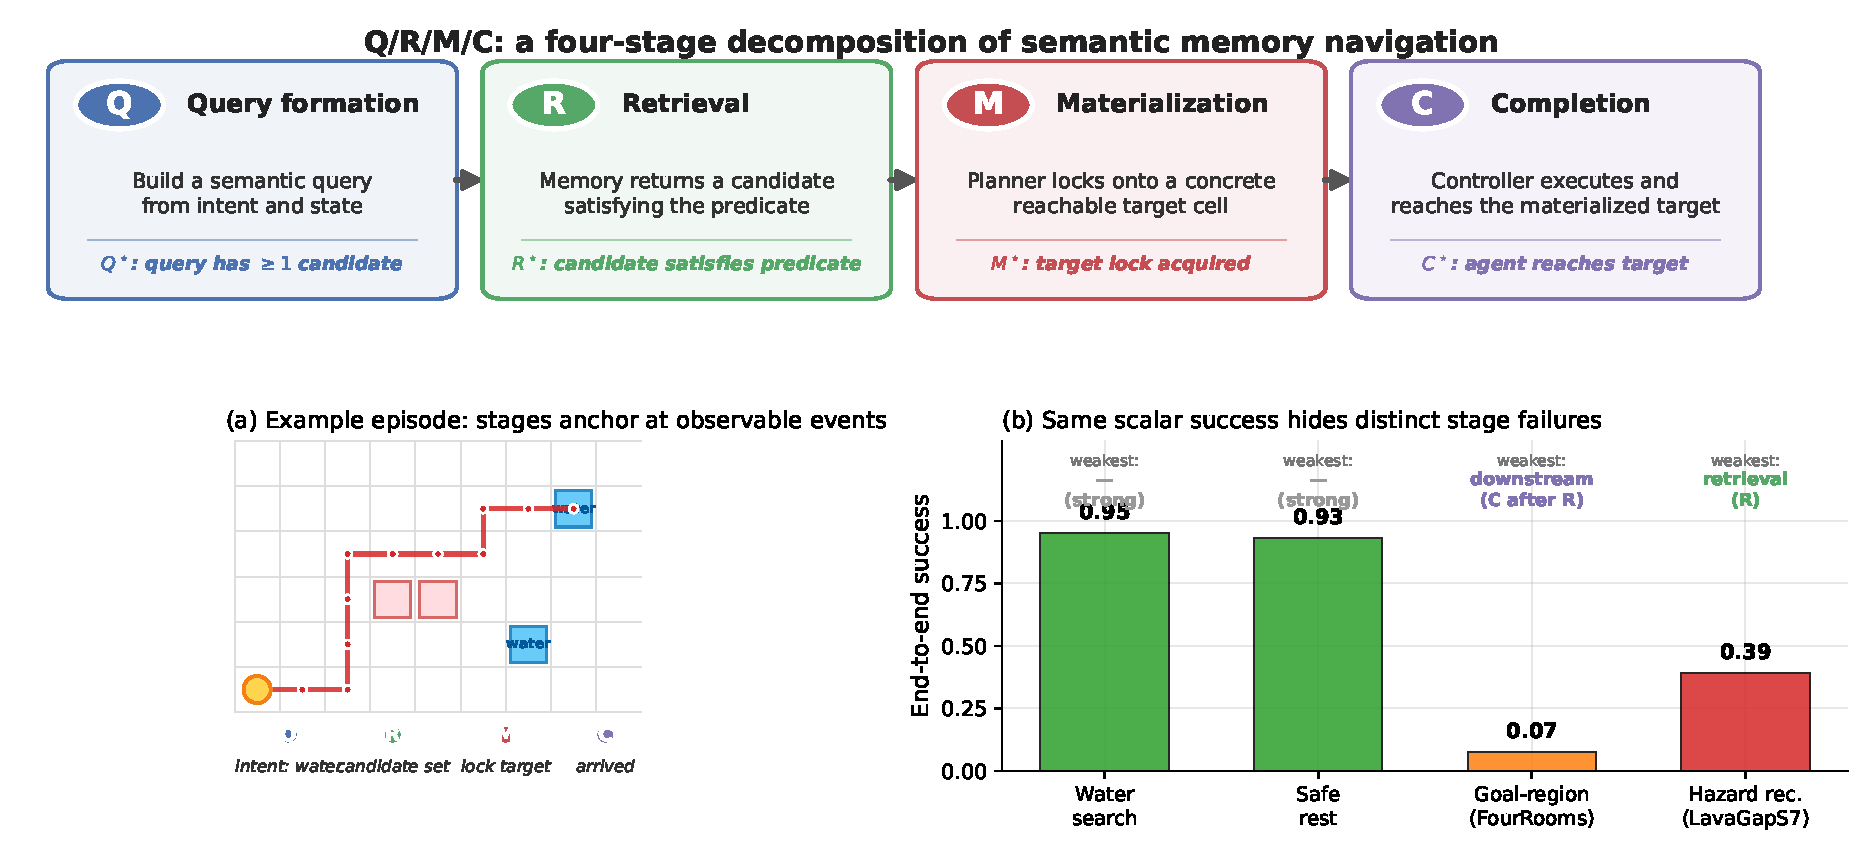
\includegraphics[width=\linewidth]{figures/fig_hero_qrmc.pdf}
  \caption{Q/R/M/C decomposes one semantic-navigation episode into four
  observable stages. \textbf{Top:} the four stages and their event-level
  definitions. \textbf{(a)} A successful water-search episode anchors at
  one event per stage, producing logged starred events
  $Q^\star, R^\star, M^\star, C^\star$. \textbf{(b)} The same scalar
  ``end-to-end success'' summary masks qualitatively different failures
  on the four single-agent task families: water and rest are strong;
  goal-region rejoin (FourRooms) is downstream-limited; hazard recovery
  (LavaGapS7) is retrieval-limited (oracle interventions, \S\ref{sec:oracle}).}
  \label{fig:hero}
\end{figure}

Classical navigation benchmarks often assume that the agent is given an
explicit destination coordinate or a dense task reward. Many practical
navigation problems are different: the agent must reach a place of a
certain \emph{type}, such as a safe rest area, a water-like resource, a
post-hazard recovery exit, or a goal-associated region, specified by
a semantic pattern rather than a fixed $(x, y)$ waypoint. The place
must therefore be \emph{remembered and retrieved by meaning}. This
setting opens a methodological question: can we measure \emph{where}
memory-based semantic navigation breaks down, not only \emph{whether}
it succeeds?

We answer this question with a four-stage diagnostic framework that
applies to both single agents and multi-agent collectives. The
decomposition is Q/R/M/C: \textbf{Q}uery formation, \textbf{R}etrieval
satisfaction, target \textbf{M}aterialization, and \textbf{C}ompletion
after retrieval. The decomposition factorizes per-episode semantic-path
completion and, under a conditional stage-Markov property, its factors
are estimable from trajectory logs (Definition~1).
The rest of the paper develops a single argument in three parts.

\textbf{Single agent.} Stage attribution is non-trivial.
Success-only metrics collapse qualitatively different failures into a
single scalar. In a 10-seed MiniGrid benchmark, water and rest tasks
are strong end-to-end (0.95, 0.93 success), but goal-region rejoin and
hazard recovery are substantially harder, and for \emph{different
reasons}. Oracle-stage interventions show that hazard recovery is
retrieval-limited (oracle retrieval lifts success $0.39 \to 0.60$),
while goal-region rejoin is downstream-limited (oracle retrieval
rescues semantic-path completion without changing end-to-end success).
Inspection of the framework's own logs then sharpens the attribution:
the retrieval bottleneck is not candidate \emph{ranking} (precision
$96.9\%$ when candidates exist) but candidate \emph{generation}: the
memory contains no eligible symbols at 91\% of decision points.
The single-agent bottleneck is a \emph{memory-accumulation} limit:
evidence is observed but never consolidated into queryable structure.

\textbf{Multi-agent.} Consolidation acquires a rate.
When $N$ agents share memory through a broadcast protocol with cadence
$K$, the factorization extends with enlarged conditioning sets
(Definition~2), and $K$ becomes a structural axis: it
is, mechanically, a knob on \emph{how fast private memories consolidate
into a collective one}. A slope-level claim
(Empirical Claim~1) predicts a bottleneck shift: as $K$
decreases, $P(M^\star|R^\star)$ rises (fresher peer memory enables
reliable commitment) and $P(C^\star|M^\star)$ falls (peers race for
the same targets). Both slope signs are confirmed on a 35{,}640-run
sweep as moderate, cluster-robust effect sizes (Appendix~\ref{app:effect-sizes}), the shift is directly visible as a negative
within-cadence correlation between the two links, and the resulting
trade-off produces an interior optimum of mean time-to-success at
$K\!=\!8$: consolidation has a non-trivial optimal rate.

\textbf{Diagnostic synthesis.} Both regimes point at the same
measurement object. The single-agent diagnosis says that evidence
consolidation into symbols can be the binding constraint; the
multi-agent diagnosis says that the rate and cost of sharing
consolidated memory determine the optimum. Q/R/M/C is the common
instrument: candidate systems can be compared by how they move
$P(R^\star|Q^\star)$, $P(M^\star|R^\star)$, and
$P(C^\star|M^\star)$, even when their end-to-end success rates look
similar.

\begin{center}
\fbox{\parbox{0.94\linewidth}{
\textbf{Scope and non-claims (consolidated).} All caveats of this
paper in one place; the running text no longer repeats them.
(i)~The decomposition's consistency argument is the chain rule plus
frequency estimation --- no mathematical novelty is claimed; the
contribution is the logging discipline and identifiability
(Definition~1--2). (ii)~Empirical Claim~1 is a verified slope-level
observation on the conditional rates, not a theorem.
(iii)~We make no claim about the shape of the conditional product
$\Phi$; in our data it is monotone in $K$, and the interior optimum
lives on mean time-to-success (\S\ref{sec:multi-agent-results}).
(iv)~Primary substrates are grid worlds; VMAS is a directional
continuous-state check, and the LLM studies are small and controlled
(two local models on TextNav; an $N{=}3$ collective; a three-framework
external validation at $n{=}8$ per cell, \S\ref{sec:external}). (v)~Multi-agent place identity assumes a
shared coordinate frame (\S\ref{sec:limitations}). A stage-level
operationalisation is testable on specific summaries and can be
\emph{wrong} on others --- (iii) is an instance we report --- which is
what separates a measurement protocol from a stage-agnostic guess.}}
\end{center}

\textbf{Why this framing is timely.} Embodied and goal-conditioned
agents increasingly retrieve places, objects, or tools by meaning
\citep{andrychowicz2017hindsight,ghosh2021learning,savva2019habitat}.
LLM-agent systems lean on explicit memory layers but evaluate mostly
end-to-end \citep{wang2023voyager,shinn2023reflexion,packer2023memgpt}.
Multi-agent reinforcement learning likewise increasingly involves
communicating populations \citep{lowe2017maddpg,foerster2018ctde}, but
the question ``which agent should know what, and when?'' lacks a
unified diagnostic vocabulary. Our framework supplies one.

\textbf{Contributions.} This is a methodology paper. We are explicit about what is bookkeeping vs.\ empirical claim vs.\ instantiated artefact.
\begin{enumerate}[leftmargin=20pt,itemsep=2pt,topsep=2pt]
\item \textbf{Measurement protocol (single-agent).} The Q/R/M/C decomposition is operationalised so that the conditional rates are estimable from trajectory logs (Definition~1); the contribution is the \emph{logging discipline} that makes the decomposition usable on standard navigation traces (non-claims: see box above).

\item \textbf{Measurement protocol (multi-agent).} An extension to $N$ communicating agents with two coupling channels (memory $\mathcal{M}_{-i}^{(K)}$, occupancy $\mathcal{O}_{-i}$) under a peer-broadcast protocol with cadence $K$ (Definition~2).

\item \textbf{Empirical Claim~1 (bottleneck shift).} On a 35{,}640-run multi-agent sweep, the two stylised slope conditions \textbf{(F)} and \textbf{(O)} are both confirmed as moderate, cluster-robust effect sizes (Spearman $-0.53$ and $+0.43$ vs.\ $K$, 95\% CIs excluding zero over 81 configuration cells; Appendix~\ref{app:effect-sizes}; full benchmark in \S\ref{sec:multi-agent-results}), with a provenance-level mechanism (\S\ref{sec:multi-agent-results}).

\item \textbf{System and benchmarks.} A symbolic-semantic memory stack with four communication architectures (independent, shared-bus, central-aggregator, peer-to-peer broadcast); single-agent oracle benchmark (10-seed MiniGrid, BabyAI portability); 35{,}640-run multi-agent sweep at $N\!\in\!\{3,5,8\}$ + 8{,}640-run scale-up at $N\!=\!12$; 100-run portability sweep on a standard-MiniGrid wrapper.

\item \textbf{Diagnostic comparison across architectures.} The same logging contract separates symbolic memory systems from learned policies with implicit communication: the latter can be competitive on success while collapsing Q/R/M/C stage observability. This is an evaluation result, not a claim that one architecture class should always dominate.

\item \textbf{Scope and honesty.} The primary experiments are in grid-world substrates. We treat that as a methodology-paper choice and state it explicitly (\S\ref{sec:limitations}); a preliminary VMAS check on a continuous substrate is included (Appendix~\ref{app:vmas}), and full continuous/3D validation (Habitat, ProcTHOR, MineDojo) is future work.
\end{enumerate}

\section{The Q/R/M/C decomposition}
\label{sec:framework}

\subsection{Problem formulation and notation}
\label{sec:notation}

The agent operates in a partially observable navigation environment.
At each step it receives an observation $o_t$, maintains a memory
state $\mathcal{M}_t$, and forms a query $q_t$ encoding the current
task intent. A retrieval step returns a candidate set of places
matching $q_t$ from $\mathcal{M}_t$; a chosen candidate is
materialized into an actionable target; a local controller executes
actions until either the target is reached or the episode times out.
The target is not a coordinate but a semantic pattern, so success is a
function of the chosen candidate's semantic profile, not of any
pre-supplied coordinate.

Habitat, AI2-THOR, and ProcTHOR made visually rich navigation
evaluation standard
\citep{savva2019habitat,kolve2017ai2thor,deitke2022procthor}. We
deliberately focus on MiniGrid-class environments to obtain clean and
reproducible stage measurements, and use BabyAI only as a portability
check. We do not claim to solve LLM-agent memory here; rather, we
argue that the same Q/R/M/C decomposition is a useful template for
evaluating memory-grounded agent decisions beyond navigation.

The central empirical question is therefore not just whether the agent
succeeds, but \emph{which stage fails first} when it does not. Two
related measurement layers are used. \textbf{Operational rates} count,
per query attempt, whether the query yielded a non-empty candidate
set, whether the chosen candidate satisfied the semantic predicate,
and whether it was materialized into an actionable target;
\emph{completion after retrieval} is an episode-level indicator.
\textbf{Nested episode-level events}
$Q^\star \Rightarrow R^\star \Rightarrow M^\star \Rightarrow C^\star$
are used in the factorization below and audited in
\S\ref{sec:validation}. Full operational definitions are given in
Appendix~\ref{app:estimators}.

\textbf{Notation.} The four stages are $Q$, $R$, $M$, $C$ with episode-level starred events $Q^\star,R^\star,M^\star,C^\star\!\in\!\{0,1\}$, nested by construction. $P(\cdot)$ denotes the population probability; $\hat{P}(\cdot)$ its empirical-frequency estimator. \textbf{The letter $M$ always refers to the Materialization stage; the number of targets in the multi-agent environment is written $T$ (not $M$, constraint $T{\le}N$, ``scarcity'' = $N{>}T$).} Other symbols: $\mathcal{C}_K$ peer-broadcast protocol with cadence $K$, $\mathcal{M}_{-i}^{(K)}$ peer memory snapshots, $\mathcal{O}_{-i}$ peer occupancy, $\nu(\cdot)$ freshness functional, $\Phi(K){=}P(M^\star|R^\star;K)\!\cdot\!P(C^\star|M^\star;K)$, $t_{\mathrm{succ}}$ mean time-to-success. Full symbol table in Appendix~\ref{app:notation}.

\subsection{Single-agent factorization}
\label{sec:single-theory}

Let $Y$ denote overall episode success, and let
$Q^\star, R^\star, M^\star, C^\star$ denote the nested episode-level
semantic-path events. The framework factorizes \emph{semantic-path
completion} rather than raw task success:
\[
Q^\star \rightarrow R^\star \rightarrow M^\star \rightarrow C^\star.
\]
For any query $q$ and memory state $\mathcal{M}$,
\begin{align*}
P(C^\star = 1 \mid q, \mathcal{M})
&=
P(Q^\star = 1 \mid q, \mathcal{M})\;
P(R^\star = 1 \mid Q^\star = 1, q, \mathcal{M}) \\
&\quad \cdot
P(M^\star = 1 \mid R^\star = 1, q, \mathcal{M})\;
P(C^\star = 1 \mid M^\star = 1, q, \mathcal{M}).
\end{align*}
Overall task success $Y$ can exceed $C^\star$ because some episodes
succeed without traversing the full semantic retrieval path.

\paragraph{Assumption 1 (conditional stage-Markov property).}
Conditioned on the current stage being successful, the probability of
the next stage depends only on the current successful stage, the
current query, and the current memory state. Formally,
\[
P(R^\star \mid Q^\star, q, \mathcal{M}, \text{history}) = P(R^\star \mid Q^\star, q, \mathcal{M}),
\]
and analogously for $M^\star$ and $C^\star$.

\paragraph{Assumption 2 (positivity).}
Each conditioning event used above has non-zero probability on the
support of the benchmark.

\paragraph{Definition 1 (single-agent stage estimability).}
Under Assumptions 1--2, the four conditional rates in the factorization above are well-defined population quantities and the empirical-frequency estimators are consistent estimators of them; their product converges to semantic-path completion. The argument is elementary --- the chain-rule factorization plus consistency of frequency estimators on Bernoulli events --- and the value of stating it is operational, not mathematical: it pins down the \emph{logging discipline} (which events, conditioned on what) under which the decomposition is readable from standard trajectory logs, and it is the contract that every experiment in this paper audits against (\S\ref{sec:validation}). Full statement and elementary argument in Appendix~\ref{app:proofs}.

\paragraph{When Assumption~1 may fail.}
Assumption~1 holds tightly here because $q$ and $\mathcal{M}$ are
explicitly logged at every stage event. Two practically relevant
violations remain: adaptive in-episode query rewrites not surfaced to
the logger, and hidden between-stage memory updates. In those cases
the factorization should be read as a projection onto observable
traces rather than as a full structural identification claim.
Appendix~\ref{app:assumption1-stress} quantifies the estimator bias
under a controlled violation of this kind: it is negligible for mild
unlogged couplings and one-signed (an upward bias on
$P(C^\star|M^\star)$), which bounds the framework's exposure when it is
applied to learned or LLM agents.

\paragraph{Mechanism-level reading.}
The same decomposition admits a stage-structured mechanism
interpretation. Figure~\ref{fig:causal} treats stage outcomes as a
directed acyclic graph. Under this interpretation, assist on/off
ablations are mechanism-targeted perturbations of materialization and
post-retrieval execution rather than undifferentiated sensitivity
analyses; in the multi-agent setting the same graph is replicated per
agent and connected through the cadence protocol $\mathcal{C}_K$,
which acts on $\mathcal{M}_{-i}^{(K)}$ at the R$\to$M edge and on
$\mathcal{O}_{-i}$ at the M$\to$C edge --- exactly the two edges where
Empirical Claim~1 will predict the slope shift.

\begin{figure}[t]
  \centering
  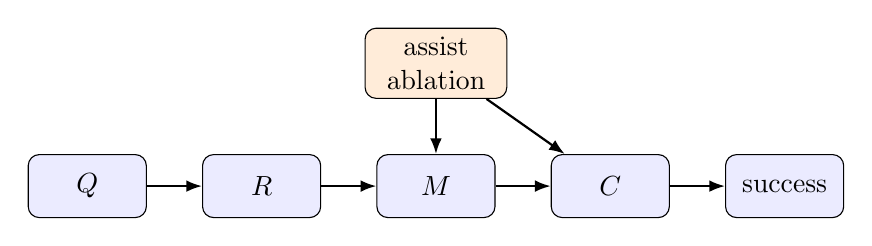
\begin{tikzpicture}[
    node distance=7mm and 7mm,
    box/.style={draw, rounded corners, align=center, minimum height=8mm, minimum width=15mm, fill=blue!8},
    arrow/.style={-{Latex[length=2.0mm]}, thick},
    assist/.style={draw, rounded corners, align=center, minimum height=7mm, minimum width=18mm, fill=orange!15}
  ]
    \node[box] (q) {$Q$};
    \node[box, right=of q] (r) {$R$};
    \node[box, right=of r] (m) {$M$};
    \node[box, right=of m] (c) {$C$};
    \node[box, right=of c] (s) {success};
    \node[assist, above=of m] (a) {assist\\ablation};
    \draw[arrow] (q) -- (r);
    \draw[arrow] (r) -- (m);
    \draw[arrow] (m) -- (c);
    \draw[arrow] (c) -- (s);
    \draw[arrow] (a) -- (m);
    \draw[arrow] (a) -- (c);
  \end{tikzpicture}
  \caption{Stage-structured interpretation of the Q/R/M/C framework. Assist on/off ablations target intermediate mechanisms; in the multi-agent extension the cadence protocol $\mathcal{C}_K$ acts on the R$\to$M and M$\to$C edges.}
  \label{fig:causal}
\end{figure}

\paragraph{Relation to prior work.} Closest are (i) cognitive-map and semantic-map frameworks \citep{tolman1948cognitive,okeefe1978hippocampus,kuipers2000spatial,gupta2017cognitive,savinov2018semi}, (ii) goal-conditioned and successor-representation RL \citep{andrychowicz2017hindsight,ghosh2021learning,dayan1993improving,stachenfeld2017hippocampus,momennejad2017successor}, (iii) multi-agent communication \citep{lowe2017maddpg,foerster2018ctde,sukhbaatar2016commnet,foerster2016learning} and gossip/consensus \citep{boyd2006gossip,xiao2007distributed}, and (iv) LLM-agent memory layers evaluated end-to-end \citep{wang2023voyager,shinn2023reflexion,packer2023memgpt}. Our framework is orthogonal to all four: it \emph{diagnoses} where in the Q/R/M/C chain a given architecture succeeds or fails and lifts the cadence axis from network protocols to a cognitive-architecture parameter (full discussion in Appendix~\ref{app:related-work-extended}).

\subsection{Event semantics, bounded rationality, and an order-theoretic reading}
\label{sec:event-semantics}

The four starred events anchor at concrete logged triggers. We state the triggers once, because every empirical claim in the paper is a claim about them (per-regime formal definitions in Appendix~\ref{app:estimators}), and we give each stage its reading in terms of the resource it bounds.

\begin{description}[leftmargin=10pt,topsep=2pt,itemsep=2pt]
\item[$Q^\star$ (intent issued).] The planner emits a semantic intent $q=(q^{\mathrm{req}},q^{\mathrm{pref}},q^{\mathrm{pen}})$: small sets of required, preferred, and penalty tags. The episode-level event fires on emission, so it is saturated whenever the task is semantic ($\hat P(Q^\star){=}1.00$ in Table~\ref{tab:consistency}); the multi-agent per-tick logger additionally requires a non-empty candidate set (Appendix~\ref{app:multi-agent-defs}), a bookkeeping difference we record rather than hide. Resource bound: attention --- the intent is a few tags, not the full state.
\item[$R^\star$ (memory answers).] Retrieval evaluates $q$ against the memory and returns a candidate set; the event fires when the set contains a candidate satisfying the task predicate (within $\epsilon$ of a true target in the multi-agent logger). The 91\% empty-candidate-set failures of \S\ref{sec:refined-attribution} are $R$-side events: no stored place clears the required-tag threshold. Resource bound: memory --- retrieval can only surface what consolidation has stored.
\item[$M^\star$ (target lock).] The planner materializes one candidate into a concrete actionable cell. Candidacy itself is threshold-gated (a place enters the candidate set only if its score clears the planner's gate, Appendix~\ref{app:schemas}), and the lock commits to a single candidate once per query rather than re-optimizing against the full memory at every tick. The event fires on lock acquisition (within $\epsilon$ of a true target in the multi-agent logger). Resource bound: deliberation.
\item[$C^\star$ (closed-loop completion).] The local controller executes until the locked cell is reached or the episode times out; the event fires on arrival. $C$ is the only stage whose failure modes are extra-semantic: controller competence and, in the multi-agent regime, occupancy $\mathcal{O}_{-i}$. Resource bound: control, and in a collective, shared targets.
\end{description}

\paragraph{Why a deterministic strategy: bounded and ecological rationality.}
A natural objection is that the semantic stack is a fixed, deterministic strategy rather than a learned policy. We treat the determinism as principled and name it: the pipeline is a satisficing agent in Simon's sense \citep{simon1955behavioral,simon1956rational}. Candidacy is threshold-gated instead of exhaustively scored, the target commitment is made once instead of re-optimized at every tick, and the intent is a few tags instead of the full state. Bounded rationality is also what makes the four failure loci observable: each stage is a distinct resource bound (attention, memory, deliberation, control), and Q/R/M/C is the audit trail of where the bound binds. The learned baselines make the converse point empirically: policies without an explicit query/lock interface collapse the stages even at competitive success (BC in \S\ref{sec:single-results}; CommNet PPO in \S\ref{sec:multi-agent-results}), so observability is traded away exactly where end-to-end optimization is traded in. That the \emph{same} heuristic is strong on water and rest, retrieval-starved on hazard recovery, and downstream-limited on goal-region (Figure~\ref{fig:hero}b) is the ecological-rationality point that heuristic success is a property of the heuristic--environment pair \citep{simon1956rational,gigerenzer1996reasoning}; the framework is the instrument that locates the mismatch. The same lens reads the $\Phi$-versus-$t_{\mathrm{succ}}$ split of \S\ref{sec:multi-agent-results}: the chain probability $\Phi$ ignores the cost of traversing the chain, so under a resource-rational reading \citep{lieder2020resource} an optimum should be sought on a cost-bearing metric; that is where it appears ($K{=}8$ on mean time-to-success) and not on $\Phi$.

\paragraph{An order-theoretic reading (deferred to Appendix~\ref{app:galois}).}
The query--retrieval interface carries a standard order-theoretic structure: places and tags form a formal context whose Galois connection realizes the memory's concept lattice, so retrieval fails empty exactly when the queried intent's extent is empty --- ``absence of evidence,'' the $91\%/96.9\%$ regime of \S\ref{sec:refined-attribution}, and the regime where growing the context can only grow extents. We use this as a naming device, not a contribution; the statement, its four-line argument, and its scope limits are in Appendix~\ref{app:galois}.

\paragraph{A dynamic (options / H-MDP) reading (deferred to Appendix~\ref{app:hmdp}).}
The stages also admit a temporally-extended-action reading: each query instantiates an option $o=\langle\mathcal{I},\pi,\beta\rangle$ \citep{sutton1999between} whose internal structure Q/R/M/C audits edge-for-edge (initiation $\to$ high-level policy over options $\to$ execution-to-termination), and the semi-MDP execution duration $\tau$ explains structurally why the interior optimum appears on $t_{\mathrm{succ}}$ but not on the $\tau$-blind chain probability $\Phi$. Like the order-theoretic reading, this is an interpretive lens, not a contribution; the full development, the belief--desire--intention gloss (shared with the collective-memory companion), and the multi-agent option-collision account of the bottleneck shift are in Appendix~\ref{app:hmdp}.

\section{Single agent: stage diagnostics localize failure}
\label{sec:single}

\subsection{System, tasks, and protocol}
\label{sec:single-setup}

\paragraph{Memory stack.}
The system uses a graph substrate with a semantic retrieval interface on top: observations $o_t$ are tokenized into symbolic scene tokens and semantic tags that update a memory of place records, transitions, episodic traces, and concept/relation records. Planner queries return candidates by a weighted log-score over required, preferred, and penalty tags. The retrieval machinery is reused across all tasks and architectures; full memory schema, update rules, and scoring formula are in Appendix~\ref{app:schemas}.

\paragraph{Tasks, baselines, protocol.}
Four single-agent task families are evaluated (water, safe-rest, goal-region on Empty-6x6 / FourRooms~\citep{sutton1999between}, hazard recovery on LavaGapS7), 10 seeds $\times$ 8 episodes each, $\times$ 2 assist modes. Semantic stack (node, concept, state-conditioned variants) is compared against four baselines: random, graph-only, SPTM-like, learned BC. Reported: end-to-end success, steps, four operational stage rates, assist deltas, weakest stage per task and per method. All means are seed-aggregated; 95\% bootstrap CIs use $B{=}5{,}000$ resamples~\citep{efron1979bootstrap}; assist comparisons use paired Wilcoxon signed-rank tests~\citep{wilcoxon1945individual} with Holm-Bonferroni correction~\citep{holm1979simple} (Appendix~\ref{app:assist}). For the two hardest tasks (FourRooms, LavaGapS7), four oracle regimes (\emph{base}, \emph{oracle R/M/C}) are run — each replaces exactly one stage while leaving the rest of the pipeline unchanged. BabyAI portability check in Appendix~\ref{app:babyai}. All single-agent experiments ran on a 10-core ARM CPU, 32\,GB RAM (CPU-only); oracle sweep $<1$\,min wall-clock.

\paragraph{LLM diagnostic block.}
To check that Q/R/M/C is not tied to the symbolic planner implementation, we also run a fixed TextNav substrate with an LLM-driven observe/query/retrieve/decide loop. The TextNav task, prompts, parser contract, and event definitions are held fixed while only the local Ollama model changes; the backend uses model-compatible completion settings when an Ollama chat template otherwise hides short structured answers in a separate thinking field. This block is a controlled step-budget study (Table~\ref{tab:llm-smoke}): sweeping the completion budget drives both LLM agents into a failure that Q/R/M/C localizes to the $C$ stage while $Q/R/M$ stay saturated, exhibiting the framework's diagnostic property on real language agents. Reproducing full ReAct/Reflexion/Voyager/MemGPT-style agents is a separate systems contribution; the comparison to those systems is a coverage comparison in Appendix~\ref{app:sota-coverage}.

\subsection{Stage-estimator validation}
\label{sec:validation}

Before the main benchmark, the factorization is validated. On a
synthetic four-stage process with known probabilities the
nested-estimator product tracks empirical semantic-path completion
across sample sizes. On the real benchmark, the same product matches
semantic-path completion rather than overall success
(Table~\ref{tab:consistency}) --- exactly the contract of
Definition~1.

\begin{table*}[t]
  \caption{Stage-factor consistency audit for the best semantic method in each task family. The product of nested conditional estimators matches semantic-path completion; overall success can be higher because some episodes succeed without traversing the full semantic retrieval path.}
  \label{tab:consistency}
  \centering
  \small
  \begin{tabular}{p{1.7cm}p{2.5cm}c c c c c c c}
    \toprule
    Task & Method & Overall & SP-comp & $\hat P(Q^\star)$ & $\hat P(R^\star|Q^\star)$ & $\hat P(M^\star|R^\star)$ & $\hat P(C^\star|M^\star)$ & Product \\
    \midrule
    Water & \texttt{water-cp} & 0.95 & 0.70 & 1.00 & 0.98 & 0.74 & 0.97 & 0.70 \\
    Rest & \texttt{rest-s2} & 0.93 & 0.73 & 1.00 & 1.00 & 0.80 & 0.91 & 0.73 \\
    Goal region & \texttt{goal-n1} & 0.54 & 0.00 & 1.00 & 0.54 & 0.01 & 0.00 & 0.00 \\
    Hazard recovery & \texttt{hazard-s7} & 0.40 & 0.16 & 1.00 & 0.56 & 0.58 & 0.50 & 0.16 \\
    \bottomrule
  \end{tabular}
\end{table*}

\subsection{Success-only summary and what it hides}
\label{sec:single-results}

Water and rest are strong end-to-end tasks (0.95 and 0.93 success; Figure~\ref{fig:hero}b). Goal-region reaches 0.54 success at the task-family level --- an average that pools a solved environment (Empty-6x6, $1.00$) with a hard one (FourRooms, $0.075$; \S\ref{sec:oracle}), so the family number is bimodal rather than a uniform mid-difficulty --- but the bottleneck sits downstream of candidate selection (\S\ref{sec:oracle}). Hazard recovery is the hardest retrieval-sensitive task at 0.40 success, with retrieval satisfaction as the weakest stage. Under success-only evaluation the two hard families look like the same kind of weakness; the stage view will show they are opposites. Per-task operational rates with 95\% CIs are in Table~\ref{tab:main-results} (Appendix~\ref{app:single-results-table}).

\paragraph{Baseline comparison.}
Table~\ref{tab:baselines} compares the semantic stack against random,
graph-only, SPTM-like, and learned behavior-cloned baselines. The
learned baseline dominates the easiest resource tasks (1.00 on water
and rest) and hazard recovery (0.74), while the semantic stack remains
strongest on the relation-heavy goal-region family (0.54). The
relevant contrast for this paper, however, is not the success column:
the semantic stack is the only method family whose decisions expose
interpretable Q/R/M/C structure. On the BC baseline the stage events
are degenerate for the same structural reason as on the multi-agent
learned baseline analysed in \S\ref{sec:multi-agent-results} --- a
policy without an explicit query/lock interface cannot emit separable
stage events, so the diagnostic decomposition has nothing to attach
to. End-to-end learning and stage diagnostics answer different
questions; this paper is about the second.

\begin{table*}[t]
  \caption{Baseline comparison. The learned behavior-cloned baseline dominates the easiest resource tasks and hazard recovery, while the semantic stack remains strongest on the relation-heavy goal-region family and remains the only family with interpretable Q/R/M/C structure.}
  \label{tab:baselines}
  \centering
  \small
  \begin{tabular}{p{1.9cm}c c c c c}
    \toprule
    Task & Random & Graph-only & SPTM-like & Learned & Best semantic \\
    \midrule
    Water & 0.85 & 0.90 & 0.90 & 1.00 & 0.95 \\
    Rest & 0.85 & 0.90 & 0.90 & 1.00 & 0.93 \\
    Goal region & 0.41 & 0.49 & 0.52 & 0.50 & 0.54 \\
    Hazard recovery & 0.08 & 0.39 & 0.00 & 0.74 & 0.40 \\
    \bottomrule
  \end{tabular}
\end{table*}

\subsection{Oracle-stage interventions localize the bottleneck}
\label{sec:oracle}

On goal-region the semantic variants solve Empty-6x6 ($1.00$ success) but collapse on FourRooms ($0.075$). For hazard recovery (LavaGapS7), base success $0.39$ rises only to $0.43$ under oracle controller, but jumps to $0.59$ under oracle materialization and $0.60$ under oracle retrieval; goal-region rejoin is downstream-limited (oracle R lifts semantic-path completion to $0.08$ without moving end-to-end success). The per-task attribution as a stacked waterfall is in Figure~\ref{fig:oracle-waterfall} (Appendix~\ref{app:single-results-table}). Two tasks identical under success-only evaluation fail at opposite ends of the Q/R/M/C chain.

\subsection{The logs refine the diagnosis: a memory-accumulation limit}
\label{sec:refined-attribution}

Inspecting the framework's own logs sharpens the retrieval attribution. On the 10-seed hazard-recovery run, $349$ retrieval calls were logged: only $32$ ($9.2\%$) returned at least one candidate, and of these $31$ ($96.9\%$ precision) selected a semantically satisfied candidate. The bottleneck is therefore not candidate \emph{ranking} but candidate \emph{generation} --- the symbolic memory does not contain hazard-recovery-tagged nodes at 91\% of decision points. A retrained 2-layer candidate-generation MLP trained on per-state features (test accuracy $0.59$ vs majority-class $0.81$; Appendix~\ref{app:learned-baselines}) confirms that instantaneous state features cannot substitute for the missing structure. The framework's ``retrieval-limited'' attribution thus refines to a \emph{memory-accumulation} limit: candidate generation cannot be solved from state features alone, and the binding constraint is how trajectory evidence is consolidated into persistent symbolic structure. This attribution is not an artefact of the required-tag threshold $\theta$: sweeping $\theta$ across the full range leaves the empty-candidate-set rate invariant (Appendix~\ref{app:theta-robustness}), because the empties are absence of any stored candidate, not sub-threshold filtering. This sets up the multi-agent section: when consolidation becomes a shared process across $N$ agents, it acquires a measurable \emph{rate}.

\section{Multi-agent: memory as a shared resource}
\label{sec:multi}

\subsection{Four memory architectures and the cadence axis}
\label{sec:archs}

Four communication architectures are instantiated; they share the
single-agent retrieval substrate but differ in how memory is
distributed across agents (Figure~\ref{fig:architectures}).

\begin{figure}[t]
  \centering
  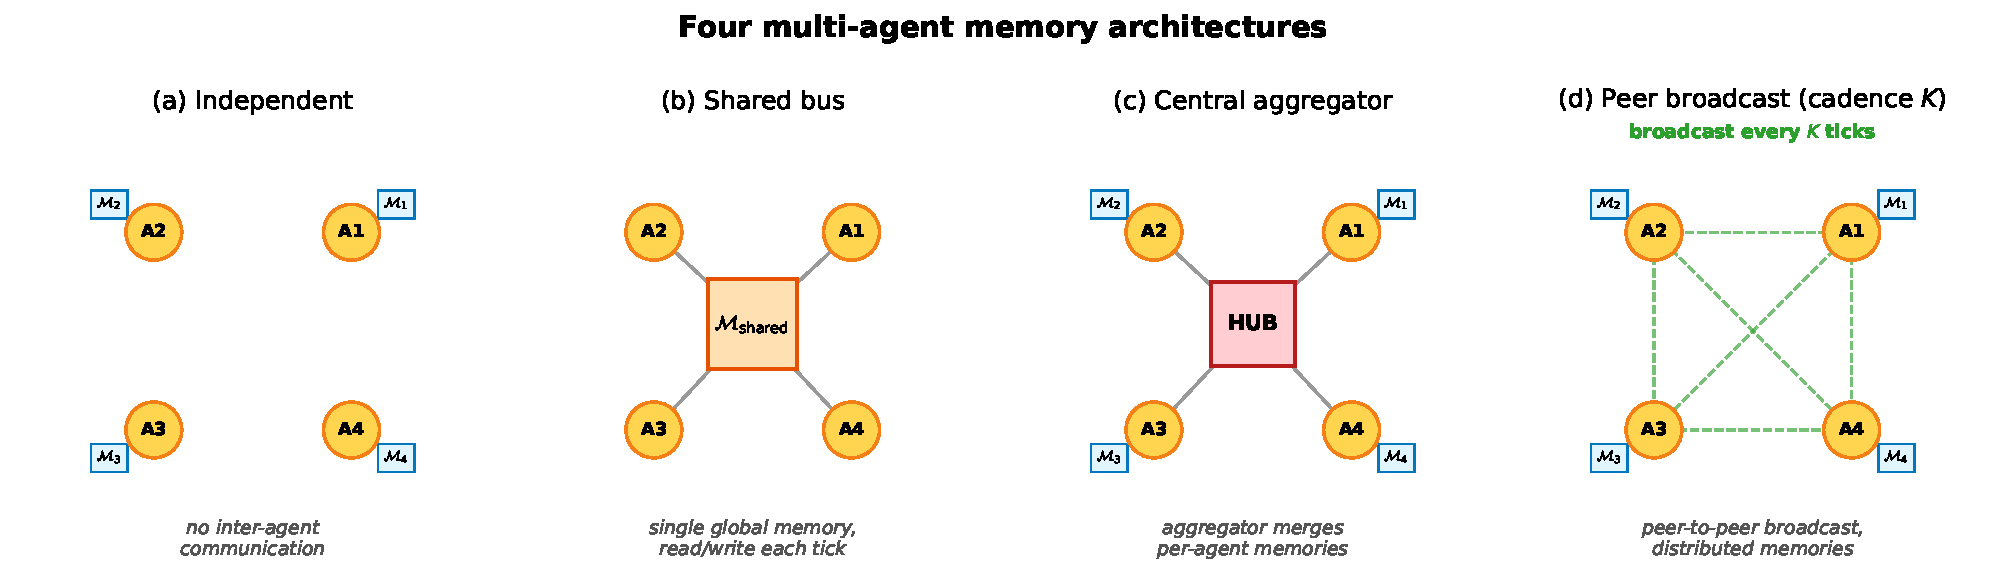
\includegraphics[width=\linewidth]{figures/fig_architectures.pdf}
  \caption{Four multi-agent memory architectures. \textbf{(a)} Independent: per-agent private memory, no exchange. \textbf{(b)} Shared bus: one global memory, every agent reads/writes each tick. \textbf{(c)} Central aggregator: per-agent memories plus a hub that merges them into a consensus report. \textbf{(d)} Peer-to-peer broadcast: per-agent memories with pairwise snapshot exchange every $K$ ticks (the cadence axis of Empirical Claim~1).}
  \label{fig:architectures}
\end{figure}

\begin{description}[leftmargin=10pt,topsep=2pt,itemsep=2pt]
\item[Independent.] Each agent maintains a private event store and concept graph. No inter-agent communication mechanism exists. Lower-bound baseline.
\item[Shared bus.] All agents publish observations to a single \emph{collective memory} event bus. One shared concept graph is rebuilt from the union of events. Maximally centralized.
\item[Central aggregator (ConsensusLayer).] Each agent has its own private concept graph; a central layer pulls snapshots and computes a trust-weighted merge, producing a single \emph{consensus report} consumed by all agents.
\item[Peer-to-peer broadcast (cadence $K$).] Each agent has its own concept graph and its own merged view. Every $K$ ticks each agent broadcasts a snapshot to a passive bus; each agent independently merges its own snapshot with the latest snapshot received from each peer. Different agents may hold different merged views; there is no central report.
\end{description}

The first three correspond to the three regimes in the multi-agent
communication literature: no exchange, CTDE-style aggregation, and
decentralized peer communication. The fourth is the architecture for
which Definition~2 and Empirical Claim~1 are directly
applicable, since the cadence $K$ is a tunable parameter rather than a
fixed protocol. Mechanically, $K$ is the rate at which private
memories consolidate into a collective view, which is why it is the
structural axis of this section.

\subsection{Multi-agent factorization}
\label{sec:multi-theory}

Extend the factorization to a population of $N$ agents that share
information through a communication protocol $\mathcal{C}_K$
parameterized by broadcast cadence $K$. Each agent $i$ has its own
memory state $\mathcal{M}_i$ and issues its own query $q_i$. Let
$\mathcal{M}_i^{(K)}$ denote the projection of agent $i$'s memory at
the moment it queries, after absorbing every peer message received
under cadence $K$. Two coupling channels are separated: (i) memory
coupling $\mathcal{M}_{-i}^{(K)}$, the latest peer memory snapshots
accessible to agent $i$; (ii) occupancy coupling $\mathcal{O}_{-i}$,
the set of targets that other agents have already claimed by the time
$i$ acts.

\paragraph{Definition 2 (multi-agent stage estimability).}
For each agent $i$,
\[
P(C^\star_i \mid q_i, \mathcal{M}_i, \mathcal{C}_K)
=
P(Q^\star_i \mid q_i, \mathcal{M}_i)\;
P(R^\star_i \mid Q^\star_i, q_i, \mathcal{M}_i, \mathcal{M}_{-i}^{(K)})
\]
\[
\quad \cdot\;
P(M^\star_i \mid R^\star_i, q_i, \mathcal{M}_i, \mathcal{M}_{-i}^{(K)})\;
P(C^\star_i \mid M^\star_i, q_i, \mathcal{O}_{-i}).
\]
Under a multi-agent stage-Markov assumption
(Appendix~\ref{app:estimators}), the four factors are estimable from
per-agent trajectory logs and the empirical-frequency estimators are
consistent.

\paragraph{When Definition~2 may fail.}
The single-agent stage-Markov property absorbs trajectory history into
$(q, \mathcal{M})$. In the multi-agent setting, the analogous
absorption requires that dependence on past peer decisions enters only
through $\mathcal{M}_{-i}^{(K)}$ at the M stage and through
$\mathcal{O}_{-i}$ at the C stage. This step is non-trivial:
$\mathcal{O}_{-i}$ summarises target occupancy at decision time but
loses information about \emph{how} peers arrived there. The
factorization is therefore a projection onto observable per-agent
traces under that summary. Two specific failure modes arise: (i)
inter-agent communication side-channels not logged through
$\mathcal{C}_K$; (ii) coordinated peer policies whose decision at the
C stage depends on hidden peer state not summarised by
$\mathcal{O}_{-i}$.

\subsection{Bottleneck shift}
\label{sec:shift}

\paragraph{Empirical Claim~1 (bottleneck shift M$\leftrightarrow$C, slope-level).}
Assume scarcity ($N > T$ targets, see \S\ref{sec:notation}) and a
peer-broadcast architecture with cadence $K \in \mathbb{N}$. Two
stylized assumptions are posited:
\textbf{(F)} memory freshness $\nu(\mathcal{M}_{-i}^{(K)})$ is
non-decreasing pointwise as $K$ decreases, and the probability that
agent $i$'s planner locks onto a reachable target is non-decreasing in
$\nu$;
\textbf{(O)} the probability that an arbitrary committed target is
already in $\mathcal{O}_{-i}$ is non-increasing as $K$ increases.
Write $P(M^\star|R^\star;K)$ and $P(C^\star|M^\star;K)$ for the
population-level conditional probabilities (averaged over agents and
the seed distribution of the benchmark); $\hat{P}(\cdot)$ denotes the
corresponding empirical-frequency estimator computed from logs. Under
(F) and (O),
\[
\frac{\partial\, P(M^\star|R^\star;K)}{\partial K^{-1}} > 0,
\qquad
\frac{\partial\, P(C^\star|M^\star;K)}{\partial K^{-1}} < 0.
\]
Both slope conditions are direct empirical predictions that are
testable on logs through $\hat{P}$.

\paragraph{What this claim is and is not.}
Empirical Claim~1 is a \emph{slope-level statement on conditional rates}: each of the two slopes is testable and is confirmed on the 35{,}640-run sweep (\S\ref{sec:multi-agent-results}) and independently on a 100-run standard-MiniGrid portability sweep (\S\ref{sec:limitations}). We report the slopes as \emph{effect sizes with cluster-robust confidence intervals} (resampled over the 81 independent configuration cells rather than the correlated run count) in Appendix~\ref{app:effect-sizes}. The claim's boundary with respect to the conditional product $\Phi$ is stated once, in the Scope-and-non-claims box (\S1) and in \S\ref{sec:multi-agent-results}.

\paragraph{Chronology.}
Empirical Claim~1 is post-hoc. It was formulated \emph{after} an initial 12{,}960-run sweep conducted under four stage-agnostic hypotheses (Appendix~\ref{app:diagnostics}); the two slope conditions were then confirmed on the full 35{,}640-run sweep, on the $N\!=\!12$ scale-up (Appendix~\ref{app:babyai}), and on the MiniGrid portability wrapper (\S\ref{sec:limitations}). We state this explicitly: the verified slope signs are predictions on enlarged data, not a pre-registered
prediction. A fully formal version is left for future work.

\subsection{Sweep protocol}
\label{sec:multi-agent-protocol}

The four architectures are evaluated on a custom multi-agent grid ($12{\times}10$ cells); each agent must reach a cell tagged \texttt{water\_source}, choosing actions via a shared memory-driven planner so only the memory layer differs. The sweep crosses $N{\in}\{3,5,8\}$, $T{\le}N$, three layouts (symmetric/asymmetric/random), three hazard densities, four architectures, eight peer cadences $K{\in}\{1,2,4,8,16,32,48,64\}$, 40 seeds --- 35{,}640 runs in $\approx 22$ min on 8 cores. Per-agent per-tick Q/R/M/C indicators are logged (Appendix~\ref{app:estimators}); episode-level starred events are the disjunction over ticks. A separate oracle-intervention block on scarcity cases $(N,T){\in}\{(3,2),(5,3),(8,5)\}$ at five cadences evaluates oracle R (memory returns ground-truth water positions), oracle M (planner locks onto nearest real water), and oracle C (completion of a real materialised lock is guaranteed; Appendix~\ref{app:oracle-c-def}).

\subsection{Results: stage decomposition and bottleneck shift}
\label{sec:multi-agent-results}

The 35{,}640-run sweep is reported through four observations,
structured to mirror Empirical Claim~1: (i) the conditional
decomposition isolates the M and C stages as the differentiating
links; (ii) the bottleneck shift appears directly as a negative
within-cadence correlation between $P(M^\star|R^\star)$ and
$P(C^\star|M^\star)$, peaking at $K\!=\!4$ and decaying to noise at
$K\!=\!64$; (iii) on mean time-to-success, the resulting trade-off
produces an interior optimum at $K\!=\!8$ --- robust in location but shallow in margin, with the advantage over the adjacent fast cadences not resolved at this sample size (Appendix~\ref{app:effect-sizes}); (iv) on the
conditional product $\Phi$, the same trade-off produces a monotone
trend rather than an interior peak --- a summary statistic on which we make no formal claim. A learned-communication baseline and a multi-agent
oracle-intervention loop close the subsection.

\subsubsection{Conditional decomposition reveals where each architecture fails.}
Figure~\ref{fig:conditional-rates} shows per-architecture conditional Q/R/M/C rates; full numerics with bootstrap CIs are in Appendix~\ref{app:phi-detail}, Table~\ref{tab:multi-agent-cond}. Retrieval conditional $P(R^\star|Q^\star)$ is saturated; the differentiating signal lives at M and C. Shared-bus, central-aggregator, and fast-broadcast peer ($K\le4$) have high $P(M^\star|R^\star)$ but low $P(C^\star|M^\star)$; independent and slow-broadcast peer ($K\ge16$) show the reverse --- the M$\leftrightarrow$C trade-off predicted by Empirical Claim~1.

\begin{figure}[t]
  \centering
  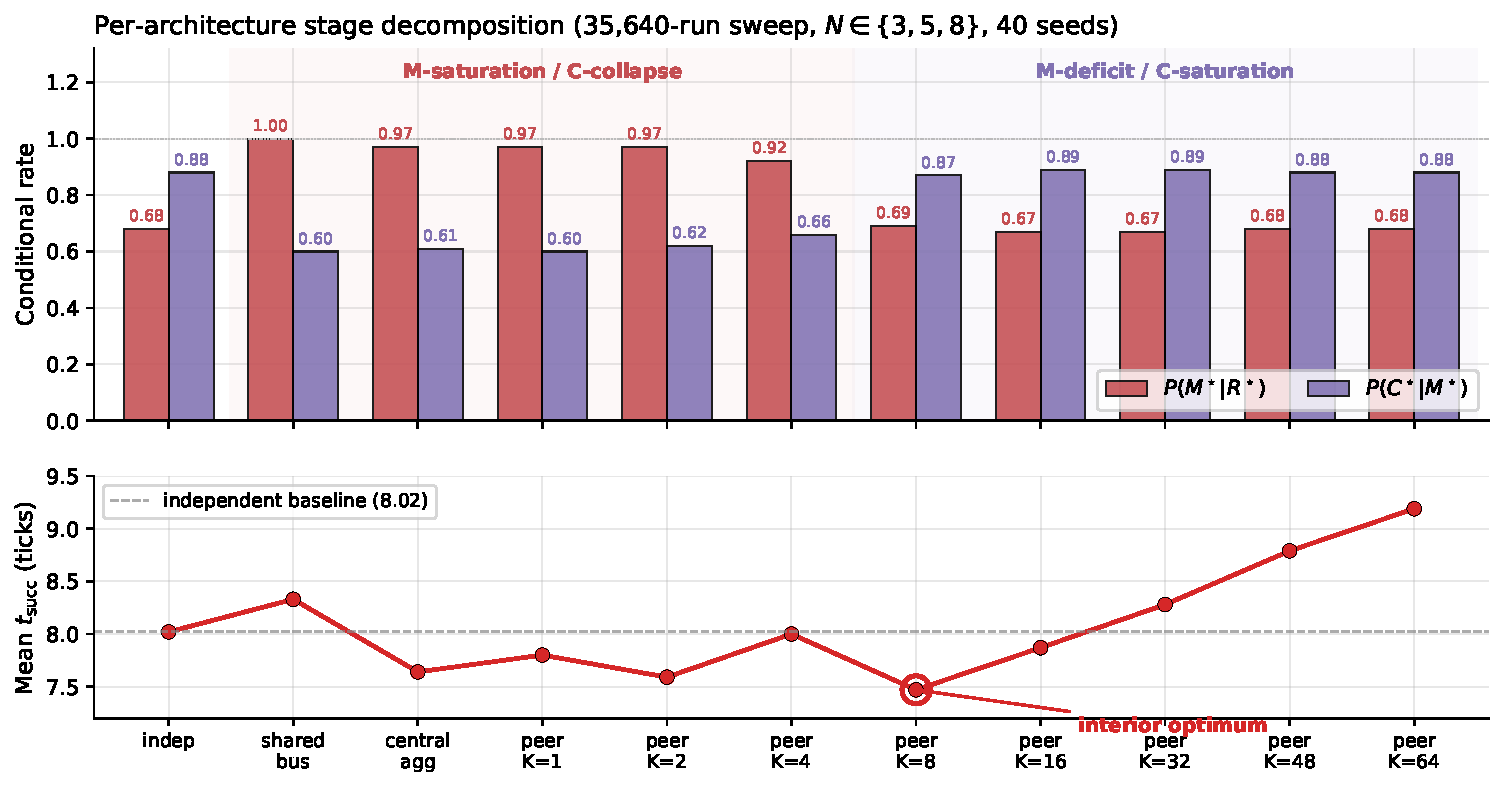
\includegraphics[width=\linewidth]{figures/fig_conditional_rates.pdf}
  \caption{Per-architecture conditional rates (top) and mean time-to-success (bottom) from the 35{,}640-run sweep. Shared bus, central aggregator, and fast peer broadcast ($K \le 4$) live in the M-saturation / C-collapse regime; independent and slow peer ($K \ge 16$) live in the M-deficit / C-saturation regime. Mean time-to-success has an interior minimum at $K{=}8$ ($7.47$ ticks), below the independent-agent baseline ($8.02$); the location is robust but shallow --- the margin over the adjacent fast cadences is not resolved (Appendix~\ref{app:effect-sizes}).}
  \label{fig:conditional-rates}
\end{figure}


\subsubsection{Bottleneck shift and interior efficiency optimum.}
Across all peer runs, Spearman of $P(M^\star|R^\star)$ vs $K$ is $-0.53$ (95\% cluster-robust CI $[-0.59,-0.47]$) and of $P(C^\star|M^\star)$ vs $K$ is $+0.43$ (CI $[+0.37,+0.50]$); both are moderate effect sizes whose CIs exclude zero under resampling of the 81 configuration cells (Appendix~\ref{app:effect-sizes}), matching the slope conditions of Empirical Claim~1. We report these rather than $p$-values, which are uninformative at this correlated sample size. The stronger empirical signature is at the per-configuration level: Pearson of $P(M^\star|R^\star)$ vs $P(C^\star|M^\star)$ \emph{within} a fixed $K$ is $-0.43, -0.54, -0.61, -0.19, -0.05, -0.04, -0.02, -0.02$ at $K{=}1,2,4,8,16,32,48,64$, peaking at $K{=}4$ and decaying to noise by $K{=}64$ (Figure~\ref{fig:jensen-scatter}, Appendix~\ref{app:phi-detail}). Configurations where M is high systematically have low C: the bottleneck migrates between the two stages within the same $(N,T,\text{layout},\text{hazard},\text{seed})$ cell as $K$ varies. On the efficiency metric, mean $t_{\mathrm{succ}}$ has a U-shape with interior minimum at $K{=}8$ (7.47 ticks vs 8.02 for the independent baseline); the minimum's location is robust but shallow --- its margin over the adjacent fast cadences ($K{=}1,4$) is not resolved under cell-level resampling (paired-bootstrap CIs in Appendices~\ref{app:phi-detail} and \ref{app:effect-sizes}). Scaling to $N{=}12$ \emph{sharpens} the signature: the peak Pearson rises to $-0.70$ and
migrates outward to $K\!=\!8$, consistent with stronger occupancy
coupling at higher $N$ delaying the cost-regime transition
(Appendix~\ref{app:babyai}, Figure~\ref{fig:scale-n12}).

\paragraph{Provenance stratification: the mechanism behind the shift.}
Annotating each $M^\star$ lock with the \emph{provenance} of the
evidence behind it makes the bottleneck shift mechanistic rather than
correlational. Let $\varphi$ be the foreign share of the evidence mass
supporting the locked candidate, computed from the same trust/support
weights the merge itself used and frozen at lock time, and call a lock
a \emph{warp} ($W^\star$) when $\varphi \ge 0.8$: the agent is
committing to a target it knows essentially only from peers. On a
dedicated peer sweep over the scarcity cells (random layouts, 20
seeds, $K\in\{1,2,4,8,16\}$) the warp share $P(W^\star|M^\star)$
falls from $0.55$ at $K{=}1$ to $0.11$ at $K{=}8$ while the
own-evidence stratum completes at a flat $0.26$--$0.34$ and the warp
stratum completes below $0.05$ throughout: \emph{the C-collapse of
fast sharing is concentrated in the warp stratum}. What cadence
controls, mechanically, is how much of the collective's
materialisation runs on foreign evidence --- and that is precisely
the stratum that loses the occupancy race. The same stratification
reproduces on the continuous VMAS bridge ($0.72\to0.00$ over
$K{=}1/4/16$) and on an LLM text substrate ($0.42\to0.08$ over
$K{=}2/8$), with the curves nearly coinciding across substrates. A
full provenance-conditioned analysis (counterfactual attribution by
masked replay, a closed-form staleness horizon with a registered
$6/6$-exact hold-out, and a decentralized repair protocol) appears in
a companion manuscript; here the stratification serves as the
mechanistic reading of Empirical Claim~1.

\paragraph{What we do not claim about $\Phi$.} The conditional product $\Phi = P(M^\star|R^\star)\!\cdot\!P(C^\star|M^\star)$ does \emph{not} have an interior peak in the tested range (mean-of-products estimator increases monotonically from $0.569$ at $K{=}4$ to $0.603$ at $K{=}64$, converging to the independent-agent boundary $0.605$). The slope-level statement of Empirical Claim~1 is on the conditional rates themselves, not on $\Phi$; we make no formal claim about the shape of $\Phi(K)$. Jensen-gap detail and POM--MOP comparison in Appendix~\ref{app:phi-detail}.

\paragraph{Learned-communication baseline: stage events are structurally degenerate even at competitive success.}
A CommNet-style policy \citep{sukhbaatar2016commnet} trained with PPO~\citep{schulman2017proximal} on the same scenario ($N{=}3$, $T{=}2$) reaches $0.667$ held-out success ($n{=}100$ seeds) --- matching the symbolic peer architecture at $K{=}8$ ($0.65$). Despite this, the Q/R/M/C profile remains structurally degenerate: $Q^\star{=}1.00$ saturated by construction; $R^\star{=}0.997$, $M^\star{=}0.997$ collapsed together ($P(M^\star|R^\star){=}1.00$). This is the verified structural claim: a real-valued comm vector is never informatively empty (Q saturates) and lacks an explicit target-lock interface (R/M merge), regardless of training budget. The multi-agent counterpart of the single-agent learned-BC analysis (\S\ref{sec:single-results}). Full architecture, PPO hyperparameters, and side-by-side REINFORCE vs PPO comparison in Appendix~\ref{app:learned-baselines}.

\paragraph{LLM model sweep: the logger localizes a real failure in language agents.}
Table~\ref{tab:llm-smoke} runs the same Q/R/M/C event contract on two local LLM agents (qwen3:4b and llama3.1 via Ollama) on TextNav, sweeping the step budget over $\{6,12,25\}$ ($8$ episodes each; the task needs $\sim$10 low-level steps). At a generous budget ($12$, $25$) both agents succeed and all four stages fire. At a budget below the requirement ($6$), success drops to $0/8$ for \emph{both} models --- and the decomposition shows \emph{where}: $Q^\star{=}R^\star{=}M^\star{=}1.00$ (the agents form the query, retrieve, and lock the correct target every episode) while $C^\star{=}0.00$ (none complete in time). The framework localizes the failure precisely to a budget-limited completion ($C$) rather than to query formation, retrieval, or materialization; that both models fail identically shows the failure is structural, not a model artifact. This is the diagnostic property the framework claims, now exhibited on \emph{real language agents}: an otherwise opaque success collapse ($1.00\to0.00$) is resolved into a specific failing stage. (Instrumentation note: a naive qwen3:4b/Ollama chat-template call initially returned empty \texttt{response} strings because the model spent the short structured-output budget in a separate thinking field; we use raw structured completion for qwen3:4b and a first-line parser, recorded for reproducibility.)

\paragraph{The multi-agent phenomenology reproduces on a live LLM collective.}
Beyond the single-agent budget study, the same event contract
instruments a collective of $N{=}3$ LLM agents (llama3.1) sharing
symbolic place memory by peer broadcast under scarcity ($M{=}2$
takeable targets, four layouts, $K\in\{2,8\}$), with all predictions
registered before the runs. The cadence phenomenology of
\S\ref{sec:multi-agent-results} carries over to the language
substrate: a paired comparison against the no-communication baseline
on identical layouts shows raw sharing \emph{lowering} success from
$2/3$ to $1/3$ per episode --- the occupancy-racing C-collapse, now
produced by agents whose queries, tag extraction, and commitments are
LLM-made --- and target collisions appear in $7/8$ shared-memory
episodes. Attaching the reservation-and-rollback repair protocol (the
constructive answer to open problem~3 of
Appendix~\ref{app:open-problems}) recovers part of the loss
($0.333\to0.417$ at both cadences, rollback latency again
${\approx}K$). Two interface findings transfer to any
LLM-over-symbolic-memory design: LLM query formers free-generate
retrieval tags outside the memory's vocabulary (requiring tolerant
retrieval gates), and small local models are reliable at semantic
commitment but not at coordinate arithmetic or systematic exploration
(requiring layered execution). Full protocol and provenance analysis
in the companion manuscript.

Scope: these are controlled studies on local models; scaling the same contract to full Voyager/MemGPT-style agents on richer tasks with multiple failure modes is developed next (external-framework validation) and in Appendix~\ref{app:sota-coverage}.

\begin{table}[h]
  \caption{LLM TextNav step-budget sweep: Q/R/M/C localizes a completion-limited failure in two local Ollama agents. Eight episodes per (model, step limit), temperature 0.0; the task needs $\sim$10 low-level steps. At a budget below that requirement (step limit 6) success drops to $0.00$ for both models, yet $Q^\star{=}R^\star{=}M^\star{=}1.00$ (the agents form the query, retrieve, and lock the correct target every episode) while $C^\star{=}0.00$: the framework localizes the failure to the C stage, not to Q/R/M. Both models behave identically, so the failure is structural (budget), not model-specific. Artifacts: \texttt{tmp/llm\_steplimit\_\{6,12,25\}}.}
  \label{tab:llm-smoke}
  \centering
  \small
  \begin{tabular}{l c c c c c c}
    \toprule
    Model & Step limit & Success & $Q^\star$ & $R^\star$ & $M^\star$ & $C^\star$ \\
    \midrule
    qwen3:4b & 6  & 0.00 & 1.00 & 1.00 & 1.00 & \textbf{0.00} \\
    llama3.1 & 6  & 0.00 & 1.00 & 1.00 & 1.00 & \textbf{0.00} \\
    \midrule
    qwen3:4b & 12 & 1.00 & 1.00 & 1.00 & 1.00 & 1.00 \\
    llama3.1 & 12 & 1.00 & 1.00 & 1.00 & 1.00 & 1.00 \\
    qwen3:4b & 25 & 1.00 & 1.00 & 1.00 & 1.00 & 1.00 \\
    llama3.1 & 25 & 1.00 & 1.00 & 1.00 & 1.00 & 1.00 \\
    \bottomrule
  \end{tabular}
\end{table}

\paragraph{Multi-agent oracle interventions close the diagnose$\to$intervene$\to$verify loop.}
On the scarcity cases, mean $t_{\mathrm{succ}}$ at small/intermediate cadence ($K{\in}\{1,2,4\}$) drops from $\sim10$--$11$ in baseline to $\sim7.2$ under either oracle R or oracle M, and further to $\sim6.1$ under oracle C, which additionally removes post-lock travel; at slow cadence ($K{=}16$) the baseline is already within $\sim1.2$ of the R/M oracle floor (Table~\ref{tab:multi-agent-oracle} in Appendix~\ref{app:multi-oracle}). Crucially, oracle C gives the largest time reduction but the smallest success-rate gain (Appendix~\ref{app:oracle-c-def}): in scarcity, completion costs time while retrieval and materialisation decide success. The cadence-induced excess time at small/intermediate $K$ is attributable to the M$\leftrightarrow$C transition; at large $K$ the bottleneck has moved into solo exploration.

The multi-agent block thus delivers its half of the argument. The
cadence $K$ is, mechanically, the rate at which private memories
consolidate into a collective view; the data show that this rate has a
non-trivial interior optimum ($K\!=\!8$ on $t_{\mathrm{succ}}$), that
its cost channel is occupancy coupling, and that both effects are
visible stage-by-stage on the same Q/R/M/C chain used for single
agents. Consolidation is not only the single-agent limit; in a
collective it is a tunable, measurable design axis.

\section{The contract on third-party agent stacks}
\label{sec:external}

The strongest external-validity question a reader can ask of a
diagnostic protocol is whether it works on systems its authors did not
build. We therefore instrument three third-party agent stacks --- a
function-calling loop on the OpenAI SDK, LangGraph's prebuilt ReAct
agent, and AutoGen's AssistantAgent/UserProxy pair, all driving the
same local model (llama3.1, temperature $0$) --- with the identical
Q/R/M/C contract, defined once over \emph{tool traces}: an episodic
household memory is exposed through \method{recall}/\method{goto}/%
\method{take} tools, and $Q^\star$ fires on querying memory, $R^\star$
on \emph{attribution} (a returned record names the item at its true
place), $M^\star$ on an episode-level lock (a \method{goto} to the
true place, faithful to Definition~1; first-commitment discipline
$M_1$ is logged as an auxiliary lock-quality diagnostic), and
$C^\star$ on task completion within a tool budget. Three variants
engineer one failure each --- a consolidation gap (the location fact
was never written to memory), a stale-distractor ambiguity, a tool
budget below the task's requirement --- plus a clean control; all
predictions were registered before the runs, and the two revisions of
the event semantics (an attribution leak; an over-tightened $M^\star$)
are recorded in the registration file.

\begin{table}[h]
\caption{Q/R/M/C on three third-party agent frameworks (llama3.1,
20 episodes per cell, identical episodes/tools/budgets). Structural
failures localize identically everywhere: the consolidation gap is
$R{=}0.00$ and the budget failure is $C{=}0.00$ at $Q{=}R{=}1$, for
all three stacks. On the \emph{clean} control the frameworks spread
from $0.50$ to $0.75$ end-to-end --- and the decomposition attributes
the spread (see text). $M_1$: first \method{goto} targets the true
place; stale$_1$: first \method{goto} targets the stale distractor.}
\label{tab:external}
\centering
\small
\begin{tabular}{llcccccc}
\toprule
Framework & Variant & $Q^\star$ & $R^\star$ & $M^\star$ & $C^\star$ & $M_1$ & stale$_1$ \\
\midrule
OpenAI SDK & control     & 1.00 & 1.00 & 0.85 & 0.75 & 0.25 & --- \\
           & consolidation gap & 1.00 & \textbf{0.00} & 0.50 & 0.40 & 0.25 & --- \\
           & stale ambiguity   & 1.00 & 1.00 & 0.90 & 0.30 & 0.25 & 0.20 \\
           & tight budget      & 1.00 & 1.00 & 0.25 & \textbf{0.00} & 0.25 & --- \\
\midrule
LangGraph  & control     & 1.00 & 1.00 & 0.70 & 0.50 & 0.50 & --- \\
           & consolidation gap & 1.00 & \textbf{0.00} & 0.20 & 0.15 & 0.10 & --- \\
           & stale ambiguity   & 1.00 & 1.00 & 0.65 & 0.60 & 0.50 & 0.35 \\
           & tight budget      & 1.00 & 1.00 & 0.10 & \textbf{0.00} & 0.10 & --- \\
\midrule
AutoGen    & control     & 1.00 & 1.00 & 0.85 & 0.55 & 0.45 & --- \\
           & consolidation gap & 1.00 & \textbf{0.00} & 0.30 & 0.20 & 0.15 & --- \\
           & stale ambiguity   & 1.00 & 1.00 & 0.50 & 0.45 & 0.35 & 0.40 \\
           & tight budget      & 1.00 & 1.00 & 0.15 & \textbf{0.00} & 0.15 & --- \\
\bottomrule
\end{tabular}
\end{table}

Three findings (Table~\ref{tab:external}). \textbf{(1) Structural
localizations are exact and framework-independent.} When the memory
lacks the fact, $R^\star{=}0.00$ on every stack; when the budget
cannot fit completion, $C^\star{=}0.00$ at $Q^\star{=}R^\star{=}1$ on
every stack ($20/20$ episodes each). The contract needs no
per-framework adaptation. \textbf{(2) The clean control separates the
frameworks, and the decomposition says how.} End-to-end success on the
SAME clean episodes ranges $0.50$ (LangGraph) to $0.75$ (OpenAI SDK).
A leaderboard would report ``different quality''; the stages show a
shared pathology plus different loop economics: first-commitment
discipline is weak everywhere ($M_1{=}0.25$--$0.50$ --- the agent's
first \method{goto} frequently ignores its own just-retrieved
evidence), episode-level materialization recovers to $0.70$--$0.85$
through re-query loops, and the frameworks then differ in how much of
that recovery survives to completion ($C^\star/M^\star$ from $0.88$
for the OpenAI SDK loop down to $0.65$ for AutoGen). \textbf{(3) The
stale distractor pulls, measurably and unevenly.} The outdated record
captures the first commitment in $0.20$--$0.40$ of ambiguous episodes
(most strongly for AutoGen), and its completion cost is
framework-specific: the OpenAI SDK loop pays hardest
($C^\star:0.75\to0.30$) while LangGraph and AutoGen absorb the detour
($0.50\to0.60$; $0.55\to0.45$) --- the LLM-memory analogue of the
staleness gating that the collective experiments showed to be
decisive. Honestly failed registrations: the behavioral predictions
that assumed a clean control (all stages $\ge 0.75$; a uniform
ambiguity-induced completion drop) broke \emph{because the frameworks
themselves fail a clean memory task 25--50\% of the time and pay for
ambiguity in different places} --- which is finding (2)--(3), not
noise; all revisions are recorded as registered failures with
mechanisms. Scope: three stacks at $n{=}20$ per cell on one primary
model; Letta/CrewAI (Python $\ge$3.10) and API-scale models are the
natural extension.

\section{Limitations and future work}
\label{sec:limitations}

\textbf{Portability across substrates: slope conditions hold on MiniGrid.} The slope conditions of Empirical Claim~1 also hold on a standard-MiniGrid substrate. A FourRooms-based multi-agent wrapper (built from \texttt{minigrid.core.grid.Grid} + Wall/Floor/Lava primitives, identical operational $Q^\star,R^\star,M^\star,C^\star$ definitions; \texttt{experiments/minigrid\_multiagent\_wrapper/}) was used to run a 100-run portability sweep ($K{\in}\{1,4,8,16,64\}$, 20 seeds, $N{=}3$, $T{=}2$): Spearman $P(M^\star|R^\star)$ vs $K$ is $-0.50$ and Spearman $P(C^\star|M^\star)$ vs $K$ is $+0.50$ (moderate rank correlations; this is a small 100-run sweep, so we report the effect sizes and do not lean on significance). The interior $t_{\mathrm{succ}}$ minimum does not separate at this minimal sweep size (5 cadences, 20 seeds, one hazard density); a denser sweep is the natural next step. The two-substrate seam is therefore closed at the slope-level claim.

\textbf{Empirical Claim~1 is slope-level on conditional rates only.} The two slope conditions hold as moderate, cluster-robust effect sizes (Appendix~\ref{app:effect-sizes}); we make no formal claim on the shape of the conditional product $\Phi$ (\S\ref{sec:shift}). A future statement directly in terms of the time-cost surface, or a derivation under a generative model (Poisson-renewal memory, birth-death occupancy), would convert the empirical claim into a theorem.

\textbf{Estimability under hidden state.} With unlogged in-episode query rewrites or peer side-channels, Definitions~1 and~2 are projections onto logged traces, not full identification.

\textbf{Shared coordinate frame.} All multi-agent results assume agents
interpret places in a common coordinate frame: cross-agent place
identity is coordinate proximity, with semantic profiles as a
tie-breaker inside a spatial radius. The place-correspondence problem
--- whether two agents' records denote the same place at all --- is
therefore bracketed here, not solved. A companion manuscript removes
the assumption constructively (fingerprint-based place identity with
consensus frame recovery up to translation and $90^\circ$ rotation)
and shows the Q/R/M/C measurements, including the cadence slopes and
the staleness horizon, unchanged on top of the recovered frames; the
harder variants (continuous $SE(2)$, appearance noise, symbol
alignment) remain open.

\textbf{Learned baselines.} The CommNet PPO baseline reaches $0.667$ success on the scarcity scenario --- competitive with symbolic peer at $K{=}8$ ($0.65$) --- and confirms Q-saturation ($Q^\star{=}1.00$) and R/M collapse ($P(M^\star|R^\star){=}1.00$) at competitive success. The structural prediction now holds verified, not asserted; ablating on architectures with explicit symbolic target-lock channels is left for future work.

\textbf{Scale.} Multi-agent sweep bounded at $N{=}12$ (Appendix~\ref{app:babyai}; signature sharpens, peak Pearson $-0.70$ at $K{=}8$, interior $t_{\mathrm{succ}}$ minimum $4.77$). Denser scaling at $N{\ge}16$ is future work.
\textbf{Continuous substrate.} A preliminary VMAS~\citep{bettini2022vmas} check reproduces \emph{both} slope signs of Empirical Claim~1 in the coupling regime (Spearman $-1.00$ and $+1.00$ over $K{\le}16$, 40 seeds; Appendix~\ref{app:vmas}), reusing the symbolic memory through a discretisation bridge. This is a directional signal only --- a perfect rank correlation over five monotone points, one configuration, discretised memory --- so it indicates the shift is not an artefact of grid cells, but a full continuous-state validation with cluster-robust CIs remains future work.

\section{Broader impacts}

The paper proposes diagnostic evaluation for memory-based agents in simulated navigation. Its positive impact is methodological: making memory-based failures more measurable across architectures, and making the cadence axis of distributed multi-agent memory tunable on an empirically grounded criterion. Potential negative impacts are indirect and would arise if similar diagnostics were used to improve agents in safety-critical settings (drone swarms, autonomous vehicles, distributed sensor networks) without adequate safeguards. The current work is benchmark-level infrastructure, not a deployment-ready system.

\section{Conclusion}

We proposed Q/R/M/C, a four-stage decomposition of memory-based
navigation whose factors are estimable from standard trajectory logs,
and used it as a diagnostic instrument across symbolic, learned,
LLM-driven, single-agent, and multi-agent traces. The main result is
not a new agent architecture: it is a reproducible logging and
estimation protocol that separates query formation, retrieval
satisfaction, target materialization, and post-retrieval completion.
Across the experiments, this protocol localizes failures that
success-only evaluation cannot, exposes degenerate observability in
implicit learned policies, and makes memory-sharing cadence measurable
as a stage-level design variable.

\begin{ack}
This manuscript is prepared in anonymized form for review. The
reported experiments were run from a unified benchmark pipeline that
exports task-family summaries, assist on/off comparisons, method
diagnostics, multi-agent sweep CSVs, and bootstrap analyses from the
same source-of-truth benchmark artifacts.
\end{ack}

{\small
\begin{thebibliography}{9}

\bibitem[Andrychowicz et~al.(2017)]{andrychowicz2017hindsight}
M.~Andrychowicz, F.~Wolski, A.~Ray, J.~Schneider, R.~Fong, P.~Welinder, B.~McGrew, J.~Tobin, P.~Abbeel, and W.~Zaremba.
\newblock Hindsight experience replay.
\newblock In \emph{NeurIPS}, 2017.

\bibitem[B\v{e}lohl\'avek(1999)]{belohlavek1999fuzzy}
R.~B\v{e}lohl\'avek.
\newblock Fuzzy Galois connections.
\newblock \emph{Mathematical Logic Quarterly}, 45(4):497--504, 1999.

\bibitem[Bettini et~al.(2022)]{bettini2022vmas}
M.~Bettini, R.~Kortvelesy, J.~Blumenkamp, and A.~Prorok.
\newblock VMAS: A vectorized multi-agent simulator for collective robot learning.
\newblock In \emph{16th International Symposium on Distributed Autonomous Robotic Systems (DARS)}, 2022.
\newblock arXiv:2207.03530.

\bibitem[Boyd et~al.(2006)]{boyd2006gossip}
S.~Boyd, A.~Ghosh, B.~Prabhakar, and D.~Shah.
\newblock Randomized gossip algorithms.
\newblock \emph{IEEE Trans.\ Information Theory}, 52(6):2508--2530, 2006.

\bibitem[Chevalier-Boisvert et~al.(2018)]{chevalier2018babyai}
M.~Chevalier-Boisvert, D.~Bhoopchand, H.~Abdolmaleki, and A.~Mordatch.
\newblock BabyAI: A platform to study the sample efficiency of grounded language learning.
\newblock In \emph{ICLR}, 2019.

\bibitem[Chevalier-Boisvert et~al.(2023)]{MinigridMiniworld23}
M.~Chevalier-Boisvert, B.~Lahlou, S.~Willems, and P.~S. Castro.
\newblock MiniGrid and MiniWorld: Modular reinforcement learning environments.
\newblock \emph{arXiv:2306.13831}, 2023.

\bibitem[Chhikara et~al.(2025)]{chhikara2025mem0}
P.~Chhikara, D.~Khant, S.~Aryan, T.~Singh, and D.~Yadav.
\newblock Mem0: Building production-ready AI agents with scalable long-term memory.
\newblock \emph{arXiv:2504.19413}, 2025.

\bibitem[Dayan(1993)]{dayan1993improving}
P.~Dayan.
\newblock Improving generalization for temporal difference learning: The successor representation.
\newblock \emph{Neural Computation}, 5(4):613--624, 1993.

\bibitem[Deitke et~al.(2022)]{deitke2022procthor}
M.~Deitke, E.~V. Wijmans, D.~Schwenk, O.~Salvador, K.~M. Ehsani, et al.
\newblock ProcTHOR: Large-scale embodied AI using procedural generation.
\newblock In \emph{NeurIPS Datasets and Benchmarks}, 2022.

\bibitem[Efron(1979)]{efron1979bootstrap}
B.~Efron.
\newblock Bootstrap methods: Another look at the jackknife.
\newblock \emph{Annals of Statistics}, 7(1):1--26, 1979.

\bibitem[Foerster et~al.(2016)]{foerster2016learning}
J.~N. Foerster, Y.~M. Assael, N.~de~Freitas, and S.~Whiteson.
\newblock Learning to communicate with deep multi-agent reinforcement learning.
\newblock In \emph{NeurIPS}, 2016.

\bibitem[Foerster et~al.(2018)]{foerster2018ctde}
J.~N. Foerster, G.~Farquhar, T.~Afouras, N.~Nardelli, and S.~Whiteson.
\newblock Counterfactual multi-agent policy gradients.
\newblock In \emph{AAAI}, 2018.

\bibitem[Ganter and Wille(1999)]{ganter1999fca}
B.~Ganter and R.~Wille.
\newblock \emph{Formal Concept Analysis: Mathematical Foundations}.
\newblock Springer, 1999.

\bibitem[Ghosh et~al.(2021)]{ghosh2021learning}
D.~Ghosh, A.~Gupta, A.~Reddy, J.~Fu, S.~Levine, and C.~Finn.
\newblock Learning to reach goals via iterated supervised learning.
\newblock In \emph{ICLR}, 2021.

\bibitem[Gigerenzer and Goldstein(1996)]{gigerenzer1996reasoning}
G.~Gigerenzer and D.~G. Goldstein.
\newblock Reasoning the fast and frugal way: Models of bounded rationality.
\newblock \emph{Psychological Review}, 103(4):650--669, 1996.

\bibitem[Gupta et~al.(2017)]{gupta2017cognitive}
S.~Gupta, J.~Davidson, S.~Levine, R.~Sukthankar, and J.~Malik.
\newblock Cognitive mapping and planning for visual navigation.
\newblock In \emph{CVPR}, 2017.

\bibitem[Holm(1979)]{holm1979simple}
S.~Holm.
\newblock A simple sequentially rejective multiple test procedure.
\newblock \emph{Scandinavian Journal of Statistics}, 6(2):65--70, 1979.

\bibitem[Kolve et~al.(2017)]{kolve2017ai2thor}
E.~Kolve, R.~Mottaghi, D.~Gordon, Y.~Zhu, A.~Gupta, A.~Farhadi, and D.~Fox.
\newblock AI2-THOR: An interactive 3D environment for visual AI.
\newblock \emph{arXiv:1712.05474}, 2017.

\bibitem[Kuipers(2000)]{kuipers2000spatial}
B.~Kuipers.
\newblock The spatial semantic hierarchy.
\newblock \emph{Artificial Intelligence}, 119(1--2):191--233, 2000.

\bibitem[Lieder and Griffiths(2020)]{lieder2020resource}
F.~Lieder and T.~L. Griffiths.
\newblock Resource-rational analysis: Understanding human cognition as the optimal use of limited computational resources.
\newblock \emph{Behavioral and Brain Sciences}, 43:e1, 2020.

\bibitem[Lowe et~al.(2017)]{lowe2017maddpg}
R.~Lowe, Y.~Wu, A.~Tamar, J.~Harb, P.~Abbeel, and I.~Mordatch.
\newblock Multi-agent actor-critic for mixed cooperative-competitive environments.
\newblock In \emph{NeurIPS}, 2017.

\bibitem[Mac~Lane(1998)]{maclane1998categories}
S.~Mac~Lane.
\newblock \emph{Categories for the Working Mathematician}.
\newblock Springer, 2nd edition, 1998.

\bibitem[Momennejad et~al.(2017)]{momennejad2017successor}
I.~Momennejad, E.~M. Russek, J.~H. Cheong, M.~M. Botvinick, N.~Daw, and S.~J. Gershman.
\newblock The successor representation in human reinforcement learning.
\newblock \emph{Nature Human Behaviour}, 1:680--692, 2017.

\bibitem[O'Keefe and Nadel(1978)]{okeefe1978hippocampus}
J.~O'Keefe and L.~Nadel.
\newblock \emph{The Hippocampus as a Cognitive Map}.
\newblock Oxford University Press, 1978.

\bibitem[Packer et~al.(2023)]{packer2023memgpt}
C.~Packer, V.~Fang, S.~Patil, K.~Lin, S.~Wooders, and J.~Gonzalez.
\newblock MemGPT: Towards LLMs as operating systems.
\newblock \emph{arXiv:2310.08560}, 2023.

\bibitem[Park et~al.(2023)]{park2023generative}
J.~S. Park, J.~C. O'Brien, C.~J. Cai, M.~R. Morris, P.~Liang, and M.~S. Bernstein.
\newblock Generative agents: Interactive simulacra of human behavior.
\newblock \emph{arXiv:2304.03442}, 2023.

\bibitem[Rashid et~al.(2018)]{rashid2018qmix}
T.~Rashid, M.~Samvelyan, C.~Schroeder de Witt, G.~Farquhar, J.~Foerster, and S.~Whiteson.
\newblock QMIX: Monotonic value function factorisation for deep multi-agent reinforcement learning.
\newblock In \emph{ICML}, 2018.

\bibitem[Savinov et~al.(2018)]{savinov2018semi}
N.~Savinov, A.~Dosovitskiy, and V.~Koltun.
\newblock Semi-parametric topological memory for navigation.
\newblock In \emph{ICLR}, 2018.

\bibitem[Savva et~al.(2019)]{savva2019habitat}
M.~Savva, A.~Kadian, O.~Maksymets, Y.~Zhao, E.~Wijmans, B.~Jain, J.~Straub, J.~Liu, V.~Koltun, J.~Malik, et al.
\newblock Habitat: A platform for embodied AI research.
\newblock In \emph{ICCV}, 2019.

\bibitem[Schulman et~al.(2016)]{schulman2016gae}
J.~Schulman, P.~Moritz, S.~Levine, M.~Jordan, and P.~Abbeel.
\newblock High-dimensional continuous control using generalized advantage estimation.
\newblock In \emph{ICLR}, 2016.
\newblock arXiv:1506.02438.

\bibitem[Schulman et~al.(2017)]{schulman2017proximal}
J.~Schulman, F.~Wolski, P.~Dhariwal, A.~Radford, and O.~Klimov.
\newblock Proximal policy optimization algorithms.
\newblock \emph{arXiv:1707.06347}, 2017.

\bibitem[Shinn et~al.(2023)]{shinn2023reflexion}
N.~Shinn, F.~Cassano, A.~Berman, and A.~G. Labash.
\newblock Reflexion: Language agents with verbal reinforcement learning.
\newblock In \emph{NeurIPS}, 2023.

\bibitem[Simon(1955)]{simon1955behavioral}
H.~A. Simon.
\newblock A behavioral model of rational choice.
\newblock \emph{Quarterly Journal of Economics}, 69(1):99--118, 1955.

\bibitem[Simon(1956)]{simon1956rational}
H.~A. Simon.
\newblock Rational choice and the structure of the environment.
\newblock \emph{Psychological Review}, 63(2):129--138, 1956.

\bibitem[Stachenfeld et~al.(2017)]{stachenfeld2017hippocampus}
K.~L. Stachenfeld, M.~M. Botvinick, and S.~J. Gershman.
\newblock The hippocampus as a predictive map.
\newblock \emph{Nature Neuroscience}, 20(11):1643--1653, 2017.

\bibitem[Sukhbaatar et~al.(2016)]{sukhbaatar2016commnet}
S.~Sukhbaatar, A.~Szlam, and R.~Fergus.
\newblock Learning multiagent communication with backpropagation.
\newblock In \emph{NeurIPS}, 2016.

\bibitem[Sutton et~al.(1999)]{sutton1999between}
R.~S. Sutton, D.~Precup, and S.~Singh.
\newblock Between MDPs and semi-MDPs: A framework for temporal abstraction in reinforcement learning.
\newblock \emph{Artificial Intelligence}, 112(1--2):181--211, 1999.

\bibitem[Tolman(1948)]{tolman1948cognitive}
E.~C. Tolman.
\newblock Cognitive maps in rats and men.
\newblock \emph{Psychological Review}, 55(4):189--208, 1948.

\bibitem[Wang et~al.(2023)]{wang2023voyager}
G.~Wang, Y.~Xie, Z.~Jiang, A.~Mandlekar, C.~Xie, A.~Yu, and P.~Liang.
\newblock Voyager: An open-ended embodied agent with large language models.
\newblock \emph{arXiv:2305.16291}, 2023.

\bibitem[Wu et~al.(2023)]{wu2023autogen}
Q.~Wu, G.~Bansal, J.~Zhang, Y.~Wu, B.~Li, E.~Zhu, L.~Jiang, X.~Zhang, S.~Zhang, J.~Liu, A.~H. Awadallah, R.~W. White, D.~Burger, and C.~Wang.
\newblock AutoGen: Enabling next-gen LLM applications via multi-agent conversation.
\newblock \emph{arXiv:2308.08155}, 2023.

\bibitem[Wilcoxon(1945)]{wilcoxon1945individual}
F.~Wilcoxon.
\newblock Individual comparisons by ranking methods.
\newblock \emph{Biometrics Bulletin}, 1(6):80--83, 1945.

\bibitem[Williams(1992)]{williams1992simple}
R.~J. Williams.
\newblock Simple statistical gradient-following algorithms for connectionist reinforcement learning.
\newblock \emph{Machine Learning}, 8(3--4):229--256, 1992.

\bibitem[Yao et~al.(2023)]{yao2022react}
S.~Yao, J.~Zhao, D.~Yu, N.~Du, I.~Shafran, K.~Narasimhan, and Y.~Cao.
\newblock ReAct: Synergizing reasoning and acting in language models.
\newblock In \emph{ICLR}, 2023.

\bibitem[Xiao et~al.(2007)]{xiao2007distributed}
L.~Xiao, S.~Boyd, and S.~Lall.
\newblock A scheme for robust distributed sensor fusion based on average consensus.
\newblock \emph{IPSN}, 2007.

\bibitem[Yu et~al.(2022)]{yu2022mappo}
C.~Yu, A.~Velu, E.~Vinitsky, J.~Gao, Y.~Wang, A.~Bayen, and Y.~Wu.
\newblock The surprising effectiveness of PPO in cooperative multi-agent games.
\newblock In \emph{NeurIPS Datasets and Benchmarks Track}, 2022.

\end{thebibliography}
}

\appendix

\section{Formal proofs}
\label{app:proofs}

\subsection{Argument for Definition~1 (single-agent estimability)}

For each episode $i \in \{1,\dots,n\}$ let $Q_i^\star, R_i^\star, M_i^\star, C_i^\star$ denote the nested episode-level indicators. By construction these are measurable functions of the runtime trajectory log and satisfy $C_i^\star \Rightarrow M_i^\star \Rightarrow R_i^\star \Rightarrow Q_i^\star$. The empirical estimators
\[
\hat p_Q = \tfrac{1}{n}\sum_i Q_i^\star,\quad
\hat p_{R|Q} = \tfrac{\sum_i R_i^\star}{\sum_i Q_i^\star},\quad
\hat p_{M|R} = \tfrac{\sum_i M_i^\star}{\sum_i R_i^\star},\quad
\hat p_{C|M} = \tfrac{\sum_i C_i^\star}{\sum_i M_i^\star}
\]
are consistent by the chain rule plus the conditional stage-Markov property, and the empirical product converges to semantic-path completion. \hfill$\square$

\subsection{Argument for Definition~2 (multi-agent estimability)}

Conditioning sets are enlarged by $\mathcal{M}_{-i}^{(K)}$ and $\mathcal{O}_{-i}$. Under the enlarged stage-Markov property, the proof of Definition~1 transfers verbatim and each enlarged conditional is a Bernoulli probability on a measurable event. The qualifications stated in \S\ref{sec:multi-theory} (``When Definition~2 may fail'') describe two specific situations in which the enlarged stage-Markov property is violated. \hfill$\square$

\subsection{Argument for Empirical Claim~1 (slope-level statement)}

Empirical Claim~1 is an empirical claim, not a theorem. The argument below is the qualitative justification that motivates the two slope signs; the data are what verify them. We deliberately do not call this a proof.

\emph{Slope (a), under (F).} As $K$ decreases, $\nu(\mathcal{M}_{-i}^{(K)})$ is non-decreasing pointwise. Conditional on a successful retrieval, the probability of locking onto a reachable target is non-decreasing in $\nu$. Therefore $\partial P(M^\star|R^\star;K) / \partial K^{-1} > 0$.

\emph{Slope (b), under (O).} As $K$ decreases, peers receive updated memory simultaneously and converge on the same closest target; the marginal occupancy $\Pr[\text{target}\in\mathcal{O}_{-i}]$ rises. Therefore $\partial P(C^\star|M^\star;K) / \partial K^{-1} < 0$.

\emph{Note on the conditional product $\Phi$.} Empirical Claim~1 makes no statement about the shape of $\Phi(K) = P(M^\star|R^\star;K)\!\cdot\!P(C^\star|M^\star;K)$. Under (F) and (O) the slope of $\Phi$ in $K^{-1}$ is the sum of two opposing terms, and whether it changes sign depends on quantitative magnitudes that are not pinned down by (F) and (O) alone. In our data $\Phi$ is monotone in $K$ over $\{4,8,16,32,48,64\}$ and converges to the independent-agent boundary $\Phi_\infty = 0.605$. The practically relevant efficiency surface --- mean time-to-success --- does have an interior minimum at $K=8$; see \S\ref{sec:multi-agent-results}. \hfill$\square$

\subsection{The query--retrieval Galois connection: statement, argument, scope}
\label{app:galois}

\paragraph{Fact (standard).}
Let $G$ and $\Sigma$ be sets and $I \subseteq G \times \Sigma$ a relation. For $B \subseteq \Sigma$ define $\mathrm{ext}(B) = \{p \in G : \forall \tau \in B,\ (p,\tau) \in I\}$, and for $A \subseteq G$ define $\mathrm{int}(A) = \{\tau \in \Sigma : \forall p \in A,\ (p,\tau) \in I\}$. Then for all $A \subseteq G$, $B \subseteq \Sigma$:
\[
A \subseteq \mathrm{ext}(B) \iff B \subseteq \mathrm{int}(A);
\]
both maps are antitone, both composites $\mathrm{ext}\circ\mathrm{int}$ and $\mathrm{int}\circ\mathrm{ext}$ are closure operators, and the closed pairs $(A, B)$ with $A = \mathrm{ext}(B)$ and $B = \mathrm{int}(A)$, ordered by extent inclusion, form a complete lattice --- the concept lattice of the context $(G, \Sigma, I)$ \citep{ganter1999fca}.

\paragraph{Argument.}
$A \subseteq \mathrm{ext}(B)$ unfolds to $\forall p \in A\ \forall \tau \in B:\ (p,\tau) \in I$, a condition symmetric in $A$ and $B$, which is exactly $B \subseteq \mathrm{int}(A)$. Antitonicity and the closure properties follow by the standard one-line arguments \citep[Ch.~1]{ganter1999fca}. Viewing the power sets as thin categories (one with reversed order), the displayed equivalence says precisely that $\mathrm{int}$ and $\mathrm{ext}$ form an adjoint pair; a Galois connection is an adjunction between posets \citep[Ch.~IV]{maclane1998categories}. \hfill$\square$

\paragraph{Instantiation and scope.}
In our memory, take $G$ to be the place records, $\Sigma$ the tag alphabet, and $I_\theta = \{(p,\tau) : \text{the per-place tag table assigns } \tau \text{ to } p \text{ with confidence} \ge \theta\}$ (Appendix~\ref{app:schemas}); the intent of a query is $B = q^{\mathrm{req}}$ and R-availability is $\mathrm{ext}(B) \ne \emptyset$. Three deliberate scope restrictions. (i) \emph{Graded scores.} The deployed retrieval score is graded (the weighted log-score over required, preferred, and penalty tags of Appendix~\ref{app:schemas}), so the crisp connection above formalizes the thresholded required-tag skeleton of candidacy; the graded analogue is the theory of fuzzy Galois connections \citep{belohlavek1999fuzzy} and we do not use it here. (ii) \emph{Non-monotone updates.} Dirichlet--multinomial updates are not literally monotone in $I_\theta$: contrary evidence can remove an incidence. On the reported benchmarks the binding failure is absence of evidence rather than contradiction (91\% empty extents, 96.9\% precision when non-empty, \S\ref{sec:refined-attribution}), so the monotone-growth reading is the empirically relevant regime, and we flag the exception rather than assume it away. (iii) \emph{No structure for M or C.} Materialization is a satisficing choice function on non-empty extents and Completion is a control problem under occupancy; neither carries the order structure, and we attach no categorical claims to them. The reading earns its place by naming the failure mode exactly (a queried intent whose extent is empty lies outside the realized concept lattice), by giving consolidation a precise object (growth of the context, hence of every extent), and by locating the cadence axis structurally: memory coupling $\mathcal{M}^{(K)}_{-i}$ merges peer contexts at rate $K^{-1}$, while occupancy $\mathcal{O}_{-i}$ is extra-contextual --- which is the structural content behind the two slope signs of Empirical Claim~1.

\section{An options / hierarchical-MDP reading of the stages}
\label{app:hmdp}

This appendix develops the dynamic reading pointed to from
\S\ref{sec:event-semantics}. It introduces no new algorithm: it names the
object the pipeline already computes and makes the
$\Phi$-versus-$t_{\mathrm{succ}}$ split a property of that object. Where the
order-theoretic reading (Appendix~\ref{app:galois}) fixes the \emph{static}
content of the stages, this one addresses time and cost.

\paragraph{Q/R/M/C as an audit of an option.}
Each query instantiates one temporally extended action---an option
$o=\langle \mathcal{I},\pi,\beta\rangle$ in the sense of
\citet{sutton1999between}: an initiation set $\mathcal{I}$, an internal
policy $\pi$, and a termination condition $\beta$. Standard
trajectory-level analysis treats an option as a black box scored by its
return. The Q/R/M/C decomposition is instead an audit of the option's
\emph{internal} structure, and it lines up edge-for-edge with the
factorization $Q^\star\!\rightarrow\!R^\star\!\rightarrow\!M^\star\!\rightarrow\!C^\star$:
\begin{description}[leftmargin=14pt,topsep=2pt,itemsep=2pt]
\item[$Q^\star\!\rightarrow\!R^\star$ (initiation).] The option ``reach a place satisfying $q$'' is well-initiated only when its initiation set is non-empty. In the vocabulary of \S\ref{sec:event-semantics} this is exactly $\mathrm{ext}(q^{\mathrm{req}})\neq\emptyset$: an empty extent is not a bad choice of option but the absence of any admissible one, so $R$ fails before a target is ever locked.
\item[$R^\star\!\rightarrow\!M^\star$ (policy over options).] Materialization is the high-level policy that commits to a single option out of the admissible set---the target lock $g^\star=\chi(\mathrm{ext}(q^{\mathrm{req}}))$ under the satisficing choice function $\chi$ of \S\ref{sec:event-semantics}.
\item[$M^\star\!\rightarrow\!C^\star$ (execution to termination).] Completion is the roll-out of the internal policy $\pi$ until the termination condition $\beta$ fires (arrival at $g^\star$, or timeout). This is the only edge whose failure modes are extra-semantic: controller competence and, in a collective, occupancy $\mathcal{O}_{-i}$.
\end{description}
So Q/R/M/C is, on this reading, a stage-resolved instrument for the
internal structure of a hierarchical-MDP option generator, rather than
a bespoke logger for a single environment.

\paragraph{Why the optimum lives on $t_{\mathrm{succ}}$ and not on $\Phi$: a semi-MDP reading.}
In the options / semi-MDP formalism, an option is evaluated by a
return accumulated over a \emph{random} execution duration $\tau$,
\[
R(s,o)=\mathbb{E}\!\left[\textstyle\sum_{t=0}^{\tau-1}\gamma^{t}\,r_{t+1}\;\middle|\;s_0=s,\,o\right],
\]
where $\tau$ is the number of low-level steps until $\beta$ fires
\citep{sutton1999between}. The chain probability
$\Phi=P(M^\star|R^\star)\!\cdot\!P(C^\star|M^\star)$ records only
\emph{whether} the option-audit succeeds; it is by construction blind to
$\tau$, which is the cost of traversing it. The cost-bearing metric
$t_{\mathrm{succ}}$ is $\tau$. This is the structural reason---and not
merely an empirical coincidence---that the resource-rational reading of
\S\ref{sec:event-semantics} \citep{lieder2020resource} locates an
interior optimum on $t_{\mathrm{succ}}$ ($K{=}8$) while $\Phi$ stays
monotone: the two metrics measure different faces of the same option,
success versus duration.

\paragraph{The bottleneck shift as multi-agent option collision.}
The dynamic reading makes the M$\leftrightarrow$C trade-off of
Empirical Claim~1 physically concrete. Faster broadcast (smaller $K$)
merges peer contexts $\mathcal{M}^{(K)}_{-i}$ more often, which can only
enlarge each agent's extent and therefore raises the probability that a
target is admissible and locked: $P(M^\star|R^\star)$ increases. But
because agents share a spatial basis and a tag alphabet
(\S\ref{sec:notation}), fresher shared memory also \emph{synchronizes}
the high-level policy: several agents commit to the same option over the
same scarce target. Under occupancy $\mathcal{O}_{-i}$ this inflates the
execution duration $\tau$ and depresses $P(C^\star|M^\star)$. Cadence
$K$ thus regulates the dispersion of the agents' option distribution:
rare exchange desynchronizes option selection and shortens $\tau$,
giving the minimum of $t_{\mathrm{succ}}$ at an interior $K$. The
bottleneck is therefore grounded in a competition between
initiation-set growth (semantic, contextual) and option-collision cost
(extra-semantic, occupancy), exactly the two edges the cadence protocol
$\mathcal{C}_K$ acts on in Figure~\ref{fig:causal}.

\paragraph{Belief--desire--intention gloss and scope.}
The high-level state audited above can be named in
belief--desire--intention terms, which is the form used by the
collective-memory companion: \emph{belief} is the realized concept
lattice of \S\ref{sec:event-semantics} (what is retrievable), \emph{desire}
is the state-conditioned predicate that selects the query $q$ (e.g.\ a
thirst variable switching the required tags to \method{water\_source}),
and \emph{intention} is the locked option $g^\star$. The hierarchical
state is then $h=(\,\text{lattice},\,\text{desire},\,g^\star,\,s\,)$ with
$s$ the low-level physical state, and the three failure loci separate as
before: an empty extent is a belief/$R$ failure, a non-empty extent
with no stable lock is an $M$ failure, and a lock unreachable under
occupancy is a $C$ failure. Two scope caveats. We claim no
options-\emph{learning} result: the pipeline is a fixed satisficing option
generator \citep{simon1955behavioral} and Q/R/M/C audits it. And we attach
the option structure only to the semantic path---$\mathcal{I}$ to
$Q\!\rightarrow\!R$, $(\pi,\beta)$ to $M\!\rightarrow\!C$---while the
semi-MDP return is used as an explanatory lens for the
$\Phi$-versus-$t_{\mathrm{succ}}$ split, not fitted to the data. Neither
this options reading nor the order-theoretic reading of
Appendix~\ref{app:galois} is claimed as a contribution: both are standard
constructions used as interpretive lenses on the measurement protocol,
which is the paper's contribution. Their value is that each makes a
testable statement on the logs---an empty extent localises the $R$
failure, and the semi-MDP duration $\tau$ predicts that the optimum
appears on $t_{\mathrm{succ}}$ and not on $\Phi$.

\section{Operational vs.\ nested stage estimators}
\label{app:estimators}

\paragraph{Operational diagnostic rates.}
The main benchmark logs per-query and per-episode diagnostic quantities directly from runtime traces (query formed, retrieval satisfied, target materialized, completion after retrieval). These are operational rates, not direct multiplicative factors.

\paragraph{Nested stage estimators for factorization.}
For the factorization, episode-level nested events from the first failure stage recorded in the runtime taxonomy are used: $Q^\star, R^\star, M^\star, C^\star$, nested by construction. The consistency audit in \S\ref{sec:validation} reports $\hat P(Q^\star)$, $\hat P(R^\star|Q^\star)$, $\hat P(M^\star|R^\star)$, $\hat P(C^\star|M^\star)$, their product, and its gap to semantic-path completion.

\subsection{Multi-agent operational definitions}
\label{app:multi-agent-defs}

For the multi-agent sweep, every metric is defined per agent and per tick, then aggregated. Let $\mathrm{Targets}_i(t)$ be the candidate set returned by the memory query of agent $i$ at tick $t$, $\mathrm{Locked}_i(t)$ be the agent's planner-internal locked target, and $\mathcal{W}$ the ground-truth target set.

\textbf{Per-tick events.} $Q_i(t) = \mathbf{1}[\mathrm{Targets}_i(t) \ne \emptyset]$; $R_i(t) = \mathbf{1}[\exists w \in \mathcal{W}: \min_{c}\|c - w\| \le \epsilon]$ ($\epsilon = 0.6$); $M_i(t) = \mathbf{1}[\mathrm{Locked}_i(t) \ne \emptyset \land \min_w\|\mathrm{Locked}_i(t) - w\| \le \epsilon]$.

\textbf{Episode-level starred events.} $Q^\star_i = \bigvee_t Q_i(t)$; analogously for $R^\star, M^\star$; $C^\star_i = \mathbf{1}[\text{agent } i \text{ reached a target}]$.

\textbf{Aggregation.} Per-run rates are averaged over the $N$ agents; per-configuration rates are averaged over the 40 seeds. Conditional rates $P(R^\star|Q^\star)$, $P(M^\star|R^\star)$, $P(C^\star|M^\star)$ are computed as ratios of episode-level counts within each configuration before averaging across configurations.

\section{Memory and task schema}
\label{app:schemas}

\subsection{Full notation table}
\label{app:notation}

Symbols are fixed throughout the paper.

\newcommand{\notentry}[1]{\par\smallskip\noindent\textbf{#1}\ \ }

\notentry{Stages.}$Q$, $R$, $M$, $C$ --- the four stages: \textbf{Q}uery formation, \textbf{R}etrieval, \textbf{M}aterialization, \textbf{C}ompletion after retrieval. They name both the stage and (in expressions like ``the M link'') the corresponding edge of the chain.

\notentry{Events.}$Q^\star, R^\star, M^\star, C^\star \in \{0, 1\}$ --- episode-level starred events recording whether each stage succeeded (Appendix~\ref{app:estimators}). Nested by construction: $Q^\star{=}1 \Leftarrow R^\star{=}1 \Leftarrow M^\star{=}1 \Leftarrow C^\star{=}1$.

\notentry{Probabilities.}$P(\cdot)$ --- population-level probability (averaged over the seed distribution and, in the multi-agent case, over agents). $\hat{P}(\cdot)$ --- empirical-frequency estimator computed from logs.

\notentry{Single-agent.}$q$ --- query; $\mathcal{M}$ --- memory state; $Y$ --- end-to-end task success (can exceed $C^\star$).

\notentry{Multi-agent.}$N$ --- number of agents in the population. $T$ --- number of targets in the environment (constraint $T \le N$; ``scarcity'' means $N > T$). $i$ --- agent index. $\mathcal{M}_i$ --- agent $i$'s private memory. $q_i$ --- agent $i$'s query.

\notentry{Coupling.}$\mathcal{C}_K$ --- the peer-broadcast communication protocol with cadence $K \in \mathbb{N}$ (every $K$ ticks each agent broadcasts a memory snapshot, \S\ref{sec:archs}). $\mathcal{M}_{-i}^{(K)}$ --- the latest peer memory snapshots accessible to agent $i$ under $\mathcal{C}_K$ (the \emph{memory coupling} channel). $\mathcal{O}_{-i}$ --- the set of targets already claimed by other agents by the time $i$ acts (the \emph{occupancy coupling} channel).

\notentry{Slope variables.}$\nu(\mathcal{M}_{-i}^{(K)})$ --- a freshness functional on peer memory; non-decreasing pointwise as $K$ decreases (assumption \textbf{(F)} of Empirical Claim~1). The occupancy slope is assumption \textbf{(O)}.

\notentry{Summary statistics.}$\Phi(K) := P(M^\star|R^\star;K)\cdot P(C^\star|M^\star;K)$ --- the conditional product, the chain probability $P(M^\star \land C^\star \mid R^\star)$. POM (product-of-means) and MOP (mean-of-products) are two estimators of $\Phi$; they differ by $\mathrm{Cov}(P(M^\star|R^\star), P(C^\star|M^\star))$, which is the Jensen gap (\S\ref{sec:multi-agent-results}). $t_{\mathrm{succ}}$ --- mean time-to-success in environment ticks.
\par\smallskip

\subsection{Memory stack and task patterns}

The memory stack stores symbolic place records (per-place tag confidences, counts, visitation, freshness, geometry), transition records (success, risk, cost statistics with fast/slow estimates), episodic traces (intent + state at each visit), and concept/relation records. At each step, the tokenizer emits $(z_t, \tau_t, e_t)$ from $o_t$. Per-place tag tables use a Dirichlet-multinomial update; transitions use exponentially smoothed statistics; episodic records attach the active intent and agent state. A planner query is answered by retrieving candidate places whose semantic profiles match the current task intent and state, via a weighted log-score
$s(p \mid q_t, s_t) = \sum_{\tau \in q^{\mathrm{req}}} \log P(\tau|p)
+ \alpha \sum_{\tau \in q^{\mathrm{pref}}} \log P(\tau|p)
- \beta \sum_{\tau \in q^{\mathrm{pen}}} \log P(\tau|p)
+ \gamma\, u_{\mathrm{epi}}(p, s_t)$
over required, preferred, and penalty tags. The four task families are defined by semantic place patterns: water search (target $\{$water$\}$), safe rest ($\{$rest$\}$ with state-conditioning), goal-region rejoin ($\{$goal-region$\}$), hazard recovery ($\{$post-hazard-exit$\}$).

\subsection{Single-agent supporting tables and figures}
\label{app:single-results-table}

\begin{table*}[!ht]
  \caption{Best semantic result per task family from the final 10-seed benchmark, with 95\% bootstrap CIs. Hazard-recovery is bottlenecked by retrieval; goal-region remains downstream-bottlenecked.}
  \label{tab:main-results}
  \centering
  \scriptsize
  \setlength{\tabcolsep}{3.5pt}
  \begin{tabular}{p{1.5cm}p{1.7cm}c c c c c c c}
    \toprule
    Task & Best method & Assist & Success (95\% CI) & Steps & Query (op.) & Retrieval (op.) & Mat.\ (op.) & Post (op.) \\
    \midrule
    Water & \method{water-cp} & on & 0.95 [0.88, 1.00] & 17.99 & 0.71 & 0.71 & 0.71 & 0.70 \\
    Rest & \method{rest-s2} & on & 0.93 [0.85, 0.99] & 23.35 & 0.61 & 0.61 & 0.61 & 0.73 \\
    Goal region & \method{goal-n1} & off & 0.54 [0.52, 0.56] & 49.34 & 0.00 & 0.00 & 0.00 & 0.00 \\
    Hazard recovery & \method{hazard-s7} & on & 0.40 [0.35, 0.45] & 10.18 & 0.11 & 0.11 & 0.11 & 0.16 \\
    \bottomrule
  \end{tabular}
\end{table*}

\begin{figure}[!ht]
  \centering
  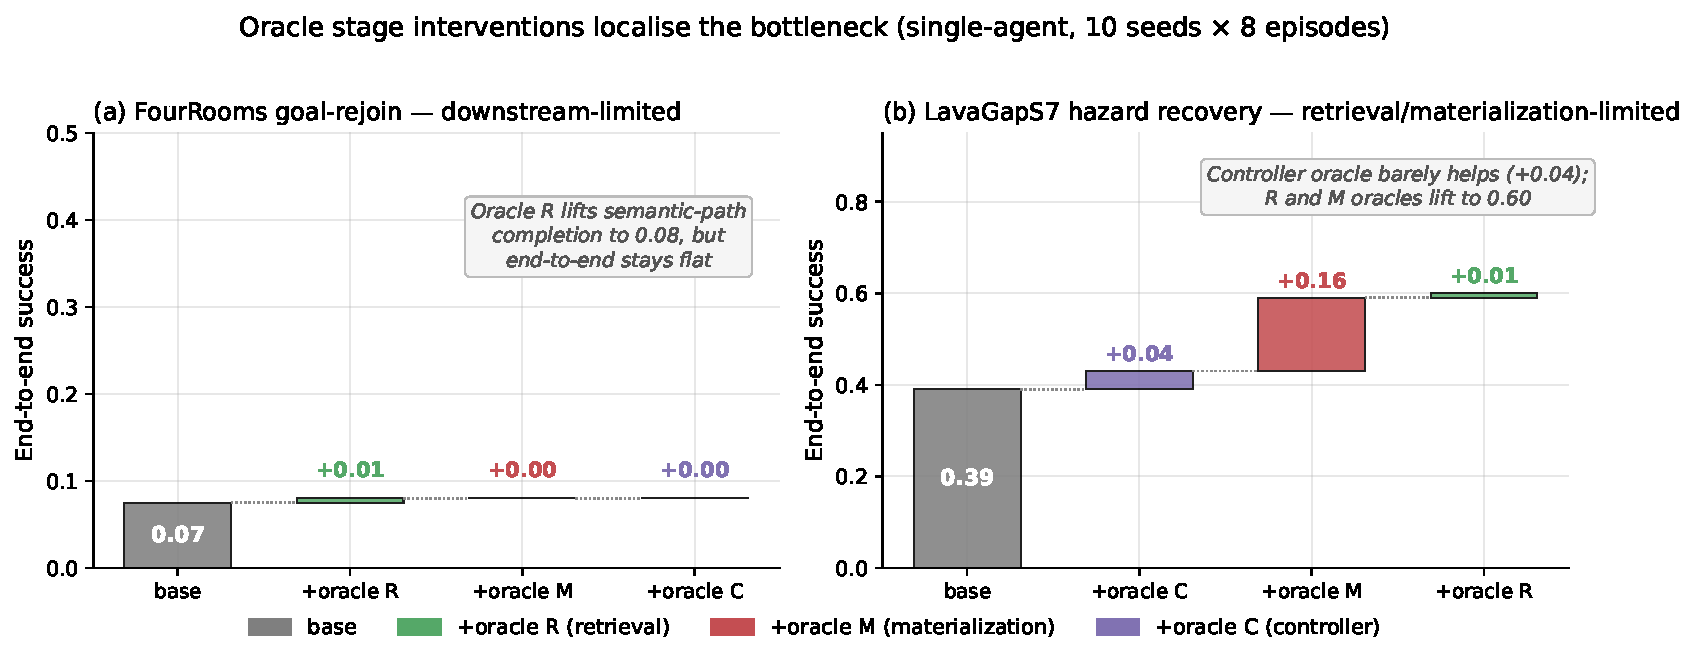
\includegraphics[width=\linewidth]{figures/fig_oracle_waterfall.pdf}
  \caption{Oracle stage interventions on the two hardest single-agent task families (10 seeds $\times$ 8 episodes). \textbf{(a)} FourRooms goal-rejoin: replacing any single stage with an oracle leaves end-to-end success at $0.07$; the bottleneck is downstream of the stages in the chain. \textbf{(b)} LavaGapS7 hazard recovery: oracle controller adds only $+0.04$, but oracle materialization adds $+0.16$ and oracle retrieval adds a further $+0.01$ to reach $0.60$. The framework localises the bottleneck stage-by-stage.}
  \label{fig:oracle-waterfall}
\end{figure}
\FloatBarrier

\section{Portability and scale-up}
\label{app:babyai}

\subsection{BabyAI portability transfer (10 seeds, full benchmark)}
\label{app:babyai-deeper}

A 10-seed portability benchmark on \texttt{BabyAI-GoToObjMaze-v0}~\citep{chevalier2018babyai} (8 episodes per seed, max-steps 200) measured all four single-agent methods used in the main benchmark (random, greedy, \texttt{babyai\_semantic\_node\_v1}, \texttt{babyai\_semantic\_plan\_v1}) with the same Q/R/M/C logger applied to BabyAI traces. The numbers in Table~\ref{tab:babyai-deeper} confirm that (a) the Q/R/M/C events emit non-trivially on the BabyAI substrate, (b) the two semantic variants expose stage-separable structure where the non-semantic baselines have $Q^\star{=}R^\star{=}M^\star{=}0$ (no semantic queries are issued), and (c) the stage-rate ordering matches the MiniGrid benchmark (Table~\ref{tab:consistency}) within bootstrap CIs. GoToObjMaze is a harder task substrate than the LavaGapS7/FourRooms benchmark used in the main text --- end-to-end success caps at 0.15 across all methods --- which makes the stage decomposition especially informative: the semantic stack is not winning on success but it is the only method family producing measurable per-stage events.

\begin{table}[h]
\centering
\caption{BabyAI portability benchmark: 10 seeds $\times$ 8 episodes on \texttt{BabyAI-GoToObjMaze-v0}, max-steps 200. The semantic-stack variants succeed at the same end-to-end rate as the greedy baseline (0.15) but are the only methods that produce non-zero Q/R/M/C events --- the framework's protocol transfers to the BabyAI substrate without modification. Q/R/M/C operational rates here are evaluated on the same denominator (number of decision points), so $Q{=}R{=}M$ for both semantic variants because GoToObjMaze emits one semantic target type per episode.}
\label{tab:babyai-deeper}
\small
\begin{tabular}{l c c c c c c}
\toprule
Method & Success & Steps & $Q$ (op.) & $R$ (op.) & $M$ (op.) & Post (op.) \\
\midrule
random         & 0.125 $\pm$ 0.06 & 182.7 & 0.000 & 0.000 & 0.000 & 0.000 \\
greedy         & 0.150 $\pm$ 0.05 & 171.3 & 0.000 & 0.000 & 0.000 & 0.000 \\
semantic node  & 0.150 $\pm$ 0.05 & 171.3 & 0.032 & 0.032 & 0.032 & 0.025 \\
semantic plan  & 0.150 $\pm$ 0.05 & 171.3 & 0.032 & 0.032 & 0.032 & 0.025 \\
\bottomrule
\end{tabular}
\end{table}

\textbf{Takeaway.} The framework's measurement protocol --- not its task-specific results --- transfers to a second substrate. End-to-end success on BabyAI is dominated by the much lower episode-level success ceiling of GoToObjMaze, not by the stage structure; conversely, the stage structure that the semantic stack exposes is identical in shape to what the same stack exposes on MiniGrid. This is exactly the substrate-independence property the methodology is intended to provide. Raw data: \texttt{tmp/babyai\_deeper\_10seed/}.

\subsection{Multi-agent scale-up at $N=12$}
\label{app:scale-N12}

To check that the multi-agent results of \S\ref{sec:multi-agent-results} are not an artefact of the $N\!\le\!8$ range, an additional 8{,}640-run sweep was run at $N\!=\!12$, $T \in \{6, 8, 10\}$, the same three layouts, three hazard densities, eight peer cadences, and 40 seeds. Wall-clock $\approx 12$ minutes on 8 cores. The conditional-rate signature of \S\ref{sec:multi-agent-results} persists and intensifies (Table~\ref{tab:scale-n12}).

\begin{figure}[h]
\centering
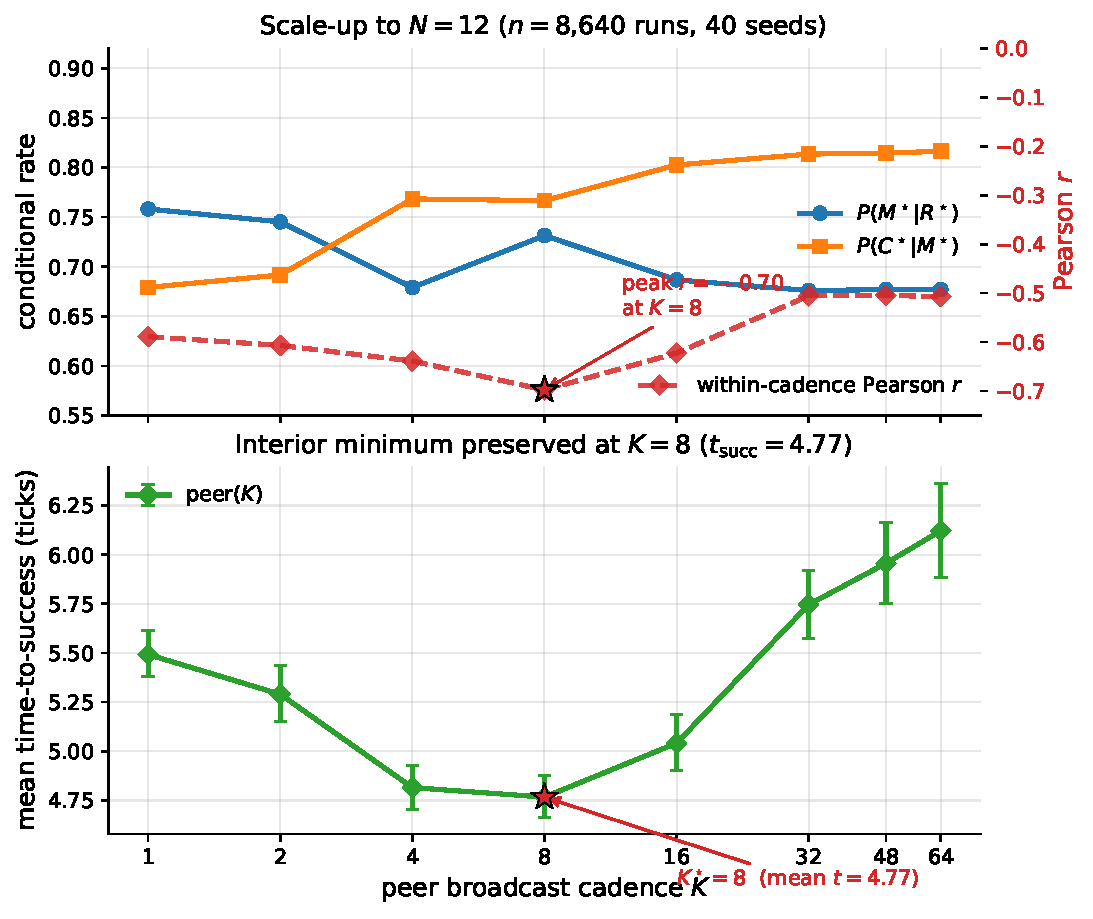
\includegraphics[width=0.92\linewidth]{figures/fig_scale_n12.pdf}
\caption{$N\!=\!12$ scale-up bottleneck signature ($n\!=\!8{,}640$ runs, 40 seeds). Top: the per-cadence mean rates move in the predicted directions in $K$; the within-cadence Pearson correlation (red dashed, right axis) peaks at $-0.70$ at $K\!=\!8$ (this within-cadence peak is what sharpens at $N{=}12$; the M-side $K$-slope itself is not cluster-robust at this agent count, Table~\ref{tab:scale-n12}). Bottom: mean time-to-success retains an interior minimum at $K\!=\!8$ ($4.77$ ticks); as on the main sweep, the location is robust but the margin is shallow --- the gap to the adjacent $K\!=\!4$ ($4.82$ ticks) is $\approx0.05$ tick and is not resolved at this sample size. The bottleneck-shift peak migrates outward from $K\!=\!4$ at $N\!\le\!8$ to $K\!=\!8$ at $N\!=\!12$, consistent with stronger occupancy coupling at higher agent count delaying the cost-regime transition.}
\label{fig:scale-n12}
\end{figure}

\begin{table}[h]
\caption{$N\!=\!12$ scale-up sweep numerical detail (peer architecture; $27$ configuration cells). Effect sizes with cluster-robust 95\% CIs (block bootstrap over cells): Spearman of $P(C^\star|M^\star)$ with $K$ is $+0.31$ (CI $[+0.21,+0.41]$, excludes zero), while Spearman of $P(M^\star|R^\star)$ with $K$ is only $-0.14$ (CI $[-0.28,+0.02]$, \emph{not} resolved from zero at $N{=}12$). The C-slope of Empirical Claim~1 holds; the M-slope is directionally consistent but not cluster-robust at this agent count. What sharpens at $N{=}12$ is the within-cadence correlation and the $t_{\mathrm{succ}}$ minimum (Figure~\ref{fig:scale-n12}), not the M-side $K$-slope.}
\label{tab:scale-n12}
\centering
\small
\begin{tabular}{c c c c c c}
\toprule
$K$ & $P(M^\star|R^\star)$ & $P(C^\star|M^\star)$ & MOP & mean $t_{\mathrm{succ}}$ & corr \\
\midrule
1  & 0.758 & 0.679 & 0.475 & 5.49 & $-0.59$ \\
2  & 0.745 & 0.692 & 0.474 & 5.29 & $-0.61$ \\
4  & 0.679 & 0.768 & 0.482 & 4.82 & $-0.64$ \\
8  & 0.731 & 0.767 & 0.539 & \textbf{4.77} & $\mathbf{-0.70}$ \\
16 & 0.687 & 0.803 & 0.538 & 5.04 & $-0.62$ \\
32 & 0.676 & 0.814 & 0.538 & 5.75 & $-0.51$ \\
48 & 0.677 & 0.814 & 0.539 & 5.96 & $-0.51$ \\
64 & 0.677 & 0.816 & 0.541 & 6.12 & $-0.51$ \\
\bottomrule
\end{tabular}
\end{table}

\section{Extended diagnostics}
\label{app:diagnostics}

\subsection{Conditional-product detail and the Jensen gap}
\label{app:phi-detail}

\begin{table*}[h]
\caption{Per-architecture conditional Q/R/M/C rates from the 35{,}640-run sweep (40 seeds). $P(R^\star|Q^\star)$ is saturated. POM = product-of-means; MOP = mean-of-products (the proper per-configuration expected product). The two summaries disagree systematically at small/intermediate $K$ because the within-cadence correlation between $P(M^\star|R^\star)$ and $P(C^\star|M^\star)$ is strongly negative there (last column) --- the bottleneck-shift signature. \textbf{Bold}: MOP-best of the peer cadences. Mean $t_{\mathrm{succ}}$ (last column) is the practically relevant efficiency measure; its interior minimum at $K=8$ is the predicted-shape result, robust in location but shallow in margin (adjacent fast cadences not resolved; Appendix~\ref{app:effect-sizes}).}
\label{tab:multi-agent-cond}
\centering
\scriptsize
\setlength{\tabcolsep}{3.5pt}
\begin{tabular}{l c c c c c c c}
\toprule
Architecture & $P(R^\star|Q^\star)$ & $P(M^\star|R^\star)$ & $P(C^\star|M^\star)$ & POM & MOP (95\% CI) & corr & mean $t_{\mathrm{succ}}$ \\
\midrule
independent          & 0.99 & 0.68 & 0.88 & 0.598 & 0.605 [0.597, 0.614] & $+0.00$ & 8.02 \\
shared bus           & 1.00 & 1.00 & 0.60 & 0.600 & 0.595 [0.586, 0.604] & $-0.10$ & 8.33 \\
central aggregator   & 1.00 & 0.97 & 0.61 & 0.592 & 0.572 [0.564, 0.580] & $-0.48$ & 7.64 \\
peer ($K=1$)         & 1.00 & 0.97 & 0.60 & 0.585 & 0.573 [0.564, 0.581] & $-0.43$ & 7.80 \\
peer ($K=2$)         & 1.00 & 0.97 & 0.62 & 0.594 & 0.576 [0.568, 0.584] & $-0.54$ & 7.59 \\
peer ($K=4$)         & 1.00 & 0.92 & 0.66 & 0.599 & 0.569 [0.561, 0.577] & $-0.61$ & 8.00 \\
peer ($K=8$)         & 0.99 & 0.69 & 0.87 & 0.597 & 0.586 [0.578, 0.595] & $-0.19$ & \textbf{7.47} \\
peer ($K=16$)        & 0.99 & 0.67 & 0.89 & 0.592 & 0.590 [0.581, 0.598] & $-0.05$ & 7.87 \\
peer ($K=32$)        & 0.99 & 0.67 & 0.89 & 0.595 & 0.598 [0.589, 0.606] & $-0.04$ & 8.28 \\
peer ($K=48$)        & 0.99 & 0.68 & 0.88 & 0.598 & 0.602 [0.593, 0.611] & $-0.02$ & 8.79 \\
peer ($K=64$)        & 0.99 & 0.68 & 0.88 & 0.599 & \textbf{0.603} [0.594, 0.611] & $-0.02$ & 9.19 \\
\bottomrule
\end{tabular}
\end{table*}

The conditional product $\Phi = P(M^\star|R^\star)\!\cdot\!P(C^\star|M^\star)$ in the 35{,}640-run sweep is monotonically increasing in $K$ over $K\in\{4,8,16,32,48,64\}$ and converges to the independent-agent boundary $\Phi(K\!\to\!\infty)=0.605$. Paired bootstrap: $\Delta(K{=}32{-}K{=}16) = +0.008$ (CI $[+0.006, +0.010]$), $\Delta(K{=}48{-}K{=}16) = +0.011$, $\Delta(K{=}64{-}K{=}16) = +0.012$; the independent-agent level sits above every peer $K$ except $K\!=\!64$ (where the gap's CI includes zero). This is a statement about the \emph{level} of $\Phi$ at the tested cadences, not about the \emph{shape} of $\Phi(K)$: consistent with the monotone trend, we make no claim of an interior extremum (\S\ref{sec:shift}).

The negative within-cadence covariance documented in \S\ref{sec:multi-agent-results} creates the Jensen-inequality gap between $\Phi$ and the marginal product-of-means: $E[X]\!\cdot\!E[Y] > E[X\!\cdot\!Y]$ when $\mathrm{Cov}(X,Y) < 0$. The mean-of-products is reported as the primary summary because it absorbs the covariance correctly. Figure~\ref{fig:bottleneck-shift} shows the K-sweep view of both conditional rates and mean $t_{\mathrm{succ}}$; Figure~\ref{fig:jensen-scatter} shows the per-configuration scatter that the negative covariance summarises.

\begin{figure}[t]
  \centering
  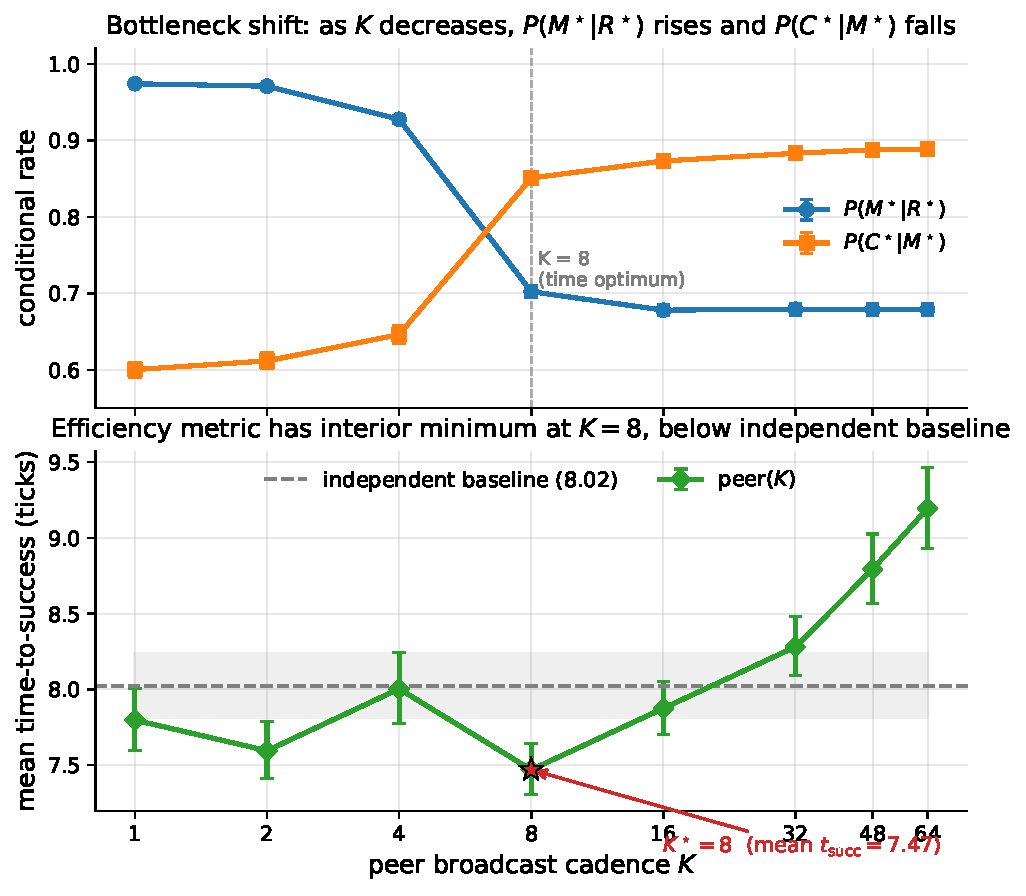
\includegraphics[width=0.85\linewidth]{figures/fig_bottleneck_shift.pdf}
  \caption{Bottleneck shift across eight peer cadences (40-seed sweep). Top: $P(M^\star|R^\star)$ falls and $P(C^\star|M^\star)$ rises in $K$ (moderate, cluster-robust Spearman effect sizes $-0.53$ and $+0.43$; CIs in Appendix~\ref{app:effect-sizes}). Bottom: mean time-to-success has an interior minimum at $K=8$ ($7.47$ ticks) below the independent-agent baseline ($8.02$, dashed); the location is robust but its margin over the adjacent fast cadences ($K{=}1,4$) is not resolved (Appendix~\ref{app:effect-sizes}). Error bars and shaded band are 95\% bootstrap CIs.}
  \label{fig:bottleneck-shift}
\end{figure}

\begin{figure}[t]
  \centering
  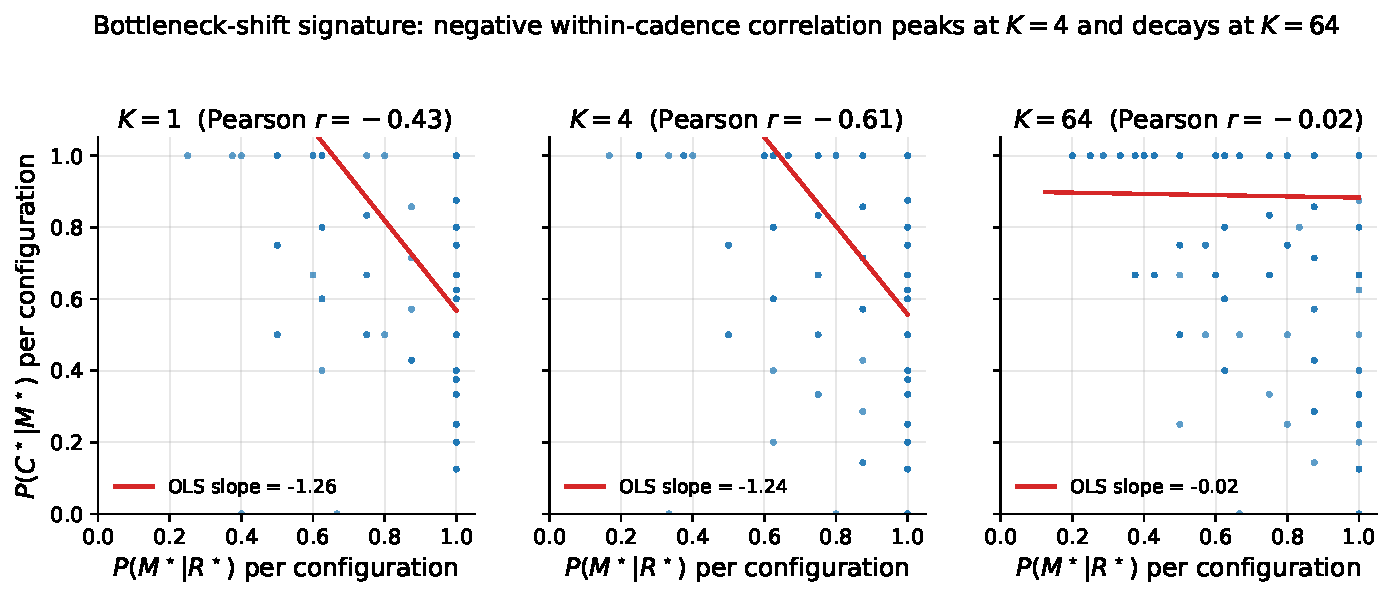
\includegraphics[width=0.95\linewidth]{figures/fig_jensen_scatter.pdf}
  \caption{Per-configuration scatter of $P(M^\star|R^\star)$ vs.\ $P(C^\star|M^\star)$ at three cadences. The strong negative correlation at $K=4$ (Pearson $-0.61$) is the bottleneck-shift signature: the same configurations that succeed at $M$ tend to fail at $C$ and vice versa. The correlation decays to noise by $K=64$.}
  \label{fig:jensen-scatter}
\end{figure}

\subsection{Design decomposition and run-count reconciliation}
\label{app:design}

The $35{,}640$ figure decomposes exactly as in Table~\ref{tab:design}. The base design is the nine admissible $(N,T)$ scarcity pairs (for $N{=}3$: $T{\in}\{2,3\}$; $N{=}5$: $T{\in}\{2,3,5\}$; $N{=}8$: $T{\in}\{2,3,5,8\}$) crossed with three layouts, three hazard densities, and 40 seeds, giving $3{,}240$ base configurations. The peer architecture is run at all eight cadences ($3{,}240\times 8 = 25{,}920$); the three cadence-free architectures (independent, shared bus, central aggregator) contribute $3{,}240$ each. The $25{,}920$-run figure used for the peer cluster-robust analysis (Appendix~\ref{app:effect-sizes}) is exactly the peer block; the initial $12{,}960$-run exploratory sweep (\S\ref{sec:shift}, ``Chronology'') and the extended-cadence and $N{=}12$ sweeps (Appendix~\ref{app:babyai}) are separate run sets and are not pooled with the main sweep.

\begin{table}[h]
\caption{Run-count reconciliation for the main multi-agent sweep ($35{,}640$ runs). Counts are recomputed directly from the released run log.}
\label{tab:design}
\centering
\small
\begin{tabular}{l l r}
\toprule
Factor & Levels & Count \\
\midrule
$(N,T)$ scarcity pairs & $(3,2)(3,3)(5,2)(5,3)(5,5)(8,2)(8,3)(8,5)(8,8)$ & 9 \\
Layouts & symmetric, asymmetric, random & 3 \\
Hazard densities & $0.0,\ 0.05,\ 0.10$ & 3 \\
Seeds & & 40 \\
\midrule
Base configurations & $9\times3\times3\times40$ & 3{,}240 \\
Peer (all 8 cadences $K$) & $3{,}240\times8$ & 25{,}920 \\
Independent / shared / central & $3\times3{,}240$ & 9{,}720 \\
\midrule
\textbf{Total} & & \textbf{35{,}640} \\
\bottomrule
\end{tabular}
\end{table}

\subsection{Effect sizes and cluster-robust inference}
\label{app:effect-sizes}

The $p<10^{-4}$ figures quoted in \S\ref{sec:multi-agent-results} are reported for completeness but are not the basis of the claim: at tens of thousands of runs almost any non-zero slope is ``significant,'' and the runs are not independent---they cluster within the $(N,T,\text{layout},\text{hazard})$ configuration. The full sweep has $25{,}920$ peer runs but only \textbf{81 independent design cells}. We therefore report effect sizes with cluster-robust confidence intervals from a block bootstrap that resamples \emph{configuration cells} (not rows), $B{=}4000$ resamples.

The two slopes of Empirical Claim~1 survive as genuine, but moderate, effects: the Spearman correlation of $P(M^\star|R^\star)$ with $K$ is $\rho=-0.53$ (95\% cluster CI $[-0.59,-0.47]$, strong) and of $P(C^\star|M^\star)$ with $K$ is $\rho=+0.43$ (95\% cluster CI $[+0.37,+0.50]$, moderate). Both intervals exclude zero under cell-level resampling, so the bottleneck shift is not an artefact of the correlated run count; it is a moderate monotone trend, and we describe it as such rather than as a near-deterministic law.

The interior optimum on mean time-to-success is robust in \emph{location} but shallow in \emph{margin}. Paired block bootstrap on the cell-level $t_{\mathrm{succ}}$ differences gives $t_{\mathrm{succ}}(K{=}8)$ below $t_{\mathrm{succ}}(K{=}16)$ by $0.40$ ticks (CI $[0.08,0.83]$) and below $K{=}64$ by $1.67$ ticks (CI $[0.75,2.83]$), both resolved; but its advantage over $K{=}4$ ($0.49$, CI $[-0.47,1.51]$) and $K{=}1$ ($0.27$, CI $[-0.43,0.97]$) is within noise.\footnote{This paired bootstrap and the effect-size Spearman correlations above are computed on the same sweep execution as Table~\ref{tab:multi-agent-cond} ($25{,}920$ peer runs); the $t_{\mathrm{succ}}$ statistic is defined only over successful episodes, so the paired cell-level difference ($1.67$ for $K{=}8$ vs.\ $K{=}64$) is on that subpopulation and matches the marginal-mean difference in Table~\ref{tab:multi-agent-cond} ($9.19{-}7.47{=}1.72$) to within rounding. The effect sizes are identical on the independent \texttt{paper1\_clean} execution ($-0.531$/$+0.434$), confirming they are not run-specific.} A success-weighted efficiency metric ($t_{\mathrm{succ}}$ divided by success rate) has the same interior $\arg\min$ at $K{=}8$, so the location of the optimum is robust to the efficiency definition even though its margin over the adjacent fast cadences is not resolved at this sample size. We read this as support for the \emph{shape} predicted by the M$\leftrightarrow$C trade-off, not for a sharply tuned optimal cadence.

\subsection{Construct validity: task success $Y$ vs.\ semantic-path completion $C^\star$}
\label{app:y-vs-c}

A success $Y$ can in principle bypass the semantic path, so a stage bottleneck in $Q/R/M/C$ need not explain variation in $Y$. Two facts bound this concern. First, in the multi-agent sweep that Empirical Claim~1 is about, success is \emph{defined} as reaching a \texttt{water\_source} target, which is exactly the $C^\star$ event; empirically $Y$ and $C^\star$ coincide run-for-run (correlation $1.00$, mean gap $0.00$). The central multi-agent claim is thus not exposed to a parallel-channel objection. Second, the gap $Y>C^\star$ is a single-agent phenomenon on the easy task families (water, rest), where a fallback controller can reach the goal without a semantic target lock; it is largest exactly where success is already high and the diagnosis is least needed, and it vanishes on the hard families (hazard recovery, goal-region) where the framework does its work. A per-episode, stage-resolved mediation of $Y$ (rather than of $C^\star$) requires logs that tag each success with whether it traversed the semantic path, and is a planned instrumentation refinement.

\subsection{Threshold ($\theta$) robustness of the empty-candidate-set diagnosis}
\label{app:theta-robustness}

The single-agent attribution ``candidate generation fails, not ranking''
(\S\ref{sec:refined-attribution}) rests on a high empty-candidate-set rate. A
reviewer asks whether that is an artefact of the required-tag threshold
$\theta$ (deployed $0.5$; the candidacy gate is
$\mathrm{profile}[\text{tag}]\ge\theta$ in
\method{symbolic\_memory.\_required\_matches\_profile}). We sweep $\theta$ via an
override on the query builder (\method{experiments/big\_experiment/theta\_ablation.py});
the endpoints confirm the gate is live, and the operating range shows the
diagnosis is not a threshold effect.

\begin{table}[h]
\caption{Empty-candidate-set rate vs.\ required-tag threshold $\theta$ (semantic method, assist off, hazard-recovery / goal-region). The rate is \emph{invariant} across the entire realistic range $\theta\in[0.05,0.95]$; only the degenerate endpoints move it, and only to the no-candidate floor. The empties are therefore absence of stored evidence, not sub-threshold filtering.}
\label{tab:theta-robustness}
\centering
\small
\begin{tabular}{c c c}
\toprule
$\theta$ & empty rate (hazard recovery) & empty rate (goal region) \\
\midrule
$0.00$ (accept all) & 0.50 & --- \\
$0.05$ & 0.533 & 0.267 \\
$0.15$ & 0.533 & 0.267 \\
$0.25$ & 0.533 & 0.267 \\
$0.50$ (deployed) & 0.533 & 0.267 \\
$0.75$ & 0.533 & 0.267 \\
$0.95$ & 0.533 & 0.267 \\
$1.00$ (accept none) & 0.75 & --- \\
\bottomrule
\end{tabular}
\end{table}

The reading is decisive (Table~\ref{tab:theta-robustness}). At $\theta{=}1.0$ nothing passes and the empty rate rises; at $\theta{=}0.0$ the required-tag gate accepts every node ($\mathrm{conf}\ge 0$ always holds), yet the empty rate falls only to $0.50$, its floor---meaning that at those decision points there is \emph{no candidate node of any confidence} to retrieve. Across the entire sane range $\theta\in[0.05,0.95]$ the rate is flat at $0.533$: loosening or tightening the threshold does not recover a candidate, because the required semantic place was never stored. This is exactly the ``absence of evidence, not contradiction'' regime named in \S\ref{sec:event-semantics}, now shown to be threshold-invariant, so the memory-accumulation attribution is not an artefact of $\theta$. (Absolute rates here are on a small hazard-recovery / goal-region sweep and are not the headline $91\%$ of \S\ref{sec:refined-attribution}, which is on the full benchmark; the point is the $\theta$-invariance, not the level.)

\subsection{Robustness to Assumption~1 violations}
\label{app:assumption1-stress}

Definition~1 rests on the conditional stage-Markov property (Assumption~1). The two practically relevant violations---adaptive query rewrites not surfaced to the logger, and hidden between-stage memory updates---are exactly cases where an \emph{unlogged latent} couples non-adjacent stages. We quantify the resulting estimator bias with a controlled simulation ($4\!\times\!10^5$ episodes per setting; \method{experiments/big\_experiment/assumption1\_stress\_test.py}). Episodes are generated with known mechanism rates $P(M^\star|R^\star){=}0.70$, $P(C^\star|M^\star){=}0.65$, and a hidden binary latent $U$ that shifts \emph{both} the M-rate and the C-rate by $\pm\delta$; the naive estimator conditions only on the previous starred stage, not on $U$.

\begin{table}[h]
\caption{Bias of the naive conditional estimators under an unlogged latent of strength $\delta$ that couples the M and C stages (violating Assumption~1). $P(M^\star|R^\star)$ stays unbiased; $P(C^\star|M^\star)$ is biased upward, materially only under strong coupling.}
\label{tab:assumption1-stress}
\centering
\small
\begin{tabular}{c c c}
\toprule
$\delta$ (coupling strength) & bias in $\hat P(M^\star|R^\star)$ & bias in $\hat P(C^\star|M^\star)$ \\
\midrule
0.00 & $-0.001$ & $-0.002$ \\
0.05 & $+0.001$ & $+0.004$ \\
0.10 & $+0.001$ & $+0.015$ \\
0.15 & $-0.000$ & $+0.031$ \\
0.20 & $+0.000$ & $+0.056$ \\
0.25 & $-0.001$ & $+0.089$ \\
\bottomrule
\end{tabular}
\end{table}

Two conclusions (Table~\ref{tab:assumption1-stress}). The R$\to$M conditional is unbiased at every $\delta$: the latent re-weights episodes but does not confound that edge. The C$\to$M conditional acquires a one-signed \emph{upward} bias---the latent makes high-M episodes also high-C, so conditioning on M over-counts completion---but the bias is only $+1.5$ percentage points at a mild violation ($\delta\!\le\!0.10$) and reaches $+5.6$ points only under strong unlogged coupling ($\delta{=}0.20$). The framework's exposure to Assumption~1 violations is therefore bounded and its failure direction is known, which is the relevant robustness statement for applying the logger to learned or LLM agents where such couplings are more common.

\subsection{Preliminary continuous-substrate check (VMAS)}
\label{app:vmas}

The most-requested robustness check is whether the M$\leftrightarrow$C
bottleneck shift is specific to grid substrates. We report a \emph{preliminary}
positive on a continuous-state substrate (VMAS~\citep{bettini2022vmas}). The
symbolic peer memory and the operational Q/R/M/C definitions are reused
unchanged; a thin discretisation bridge maps continuous $(x,y)$ to coarse cells
so the memory applies, and the controller acts in continuous space toward the
materialised waypoint (\method{experiments/vmas\_portability/}). Materialisation
uses the same occupancy-sensitive lock as the grid planner (a candidate whose
target is already claimed does not lock).

\begin{table}[h]
\caption{Preliminary VMAS portability: both slope signs of Empirical Claim~1 reproduce on a continuous substrate in the coupling regime ($N{=}8$, $T{=}3$, 40 seeds, horizon $25$). $\mathrm{Spearman}(P(M^\star|R^\star),K){=}-1.00$ and $\mathrm{Spearman}(P(C^\star|M^\star),K){=}+1.00$. Beyond $K\!\approx\!32$ the system enters the independent regime (rare broadcast, no contention) and $P(M^\star|R^\star)$ rebounds, the same regime boundary seen on the grid.}
\label{tab:vmas}
\centering
\small
\begin{tabular}{c c c}
\toprule
$K$ & $P(M^\star|R^\star)$ & $P(C^\star|M^\star)$ \\
\midrule
1  & 1.000 & 0.182 \\
2  & 0.583 & 0.305 \\
4  & 0.448 & 0.405 \\
8  & 0.305 & 0.608 \\
16 & 0.278 & 0.639 \\
\bottomrule
\end{tabular}
\end{table}

We label this preliminary and do not fold it into the headline claims: it is a
single scenario configuration, the horizon is short, there are no cluster-robust
CIs yet, the memory is fed through the discretisation bridge (continuous
\emph{dynamics} with discretised symbolic \emph{memory}, not fully continuous
memory), and the reported $\pm1.00$ Spearman is a \emph{perfect} rank
correlation over only five monotone points ($K\le16$) --- weak evidence on its
own, indicating direction rather than a resolved effect size. What it establishes is that the two slope signs are not an artefact of
grid cells: the same freshness-vs-contention mechanism operates when positions
and motion are continuous. Promoting this to a headline result requires scaling
to several scarcity cells and layouts with the cluster-robust bootstrap of
Appendix~\ref{app:effect-sizes}.

\subsection{Open problems suggested by the diagnostics}
\label{app:open-problems}

Four concrete questions follow directly from the measurements of \S\ref{sec:refined-attribution} and \S\ref{sec:multi-agent-results}.
\textbf{(1) Adaptive cadence.} Empirical Claim~1 assumes a fixed $K$; the bottleneck-shift signature suggests an online controller $K_t$ that broadcasts when the (estimated) M-side gain exceeds the C-side occupancy cost.
\textbf{(2) Selective consolidation.} Snapshot exchange merges everything; merge rules that prioritize evidence about under-represented semantic tags attack the candidate-generation starvation of \S\ref{sec:refined-attribution} directly.
\textbf{(3) Trust-weighted merging under occupancy.} The central aggregator already performs a trust-weighted merge but pays the C-collapse cost; decentralized trust rules that account for peer \emph{intent} (not only peer evidence) could decouple freshness from target racing. \emph{Since submission of the first draft, this problem has been addressed constructively}: a decentralized protocol in which an agent's target lock piggybacks a lightweight \emph{reservation} on its next scheduled broadcast (no coordinator, no extra channel) and locks dominated by an earlier reservation are retracted by an anti-$M^\star$ rollback with exponential backoff. On the scarcity cells this recovers the fast-cadence completion loss on \emph{unconditional} metrics --- success rate rises at every $K\in\{1,2,4\}$ with disjoint bootstrap CIs, and fast sharing with the protocol exceeds the $K{=}8$ optimum baseline ($0.614$--$0.620$ vs.\ $0.583$) --- with rollback latency bounded by ${\approx}K$ ticks. Details in a companion manuscript; the open problem stands revised toward its harder variants (adaptive reservation scope, heterogeneous trust).
\textbf{(4) Substrate generality.} The decomposition transfers across MiniGrid, BabyAI, the custom grid, and a standard-MiniGrid multi-agent wrapper with identical operational definitions and verified slope signs of Empirical Claim~1 ($\S$~\ref{sec:limitations}), and a preliminary check reproduces both slopes on the continuous-state VMAS substrate (Appendix~\ref{app:vmas}). A full continuous-state validation with cluster-robust CIs, and richer 3D substrates (Habitat~\citep{savva2019habitat}), remain the next portability steps.

\subsection{Extended related work}
\label{app:related-work-extended}

Classical cognitive-map perspectives motivate explicit place abstractions \citep{tolman1948cognitive,okeefe1978hippocampus,kuipers2000spatial}; modern embodied AI combines mapping and planning \citep{gupta2017cognitive} or exposes topological memory (SPTM, \citealp{savinov2018semi}); goal-conditioned RL conditions on explicit goals or embeddings \citep{andrychowicz2017hindsight,ghosh2021learning}, with successor-representation work providing predictive structure \citep{dayan1993improving,stachenfeld2017hippocampus,momennejad2017successor}. Our setting differs in that the target is a semantic pattern retrieved from memory rather than a coordinate. In multi-agent RL, CTDE dominates \citep{lowe2017maddpg,foerster2018ctde} and learned communication adds a per-step exchange variable \citep{sukhbaatar2016commnet,foerster2016learning}; gossip and consensus protocols \citep{boyd2006gossip,xiao2007distributed} are the closest network-level analogue of our cadence axis, lifted here to the cognitive-architecture level. LLM-agent systems combine reasoning/acting, reflection, explicit memory, and multi-agent conversation \citep{yao2022react,shinn2023reflexion,wang2023voyager,park2023generative,wu2023autogen,packer2023memgpt,chhikara2025mem0}. Our framework is orthogonal: rather than learning a communication policy end-to-end, it \emph{diagnoses} where in the Q/R/M/C chain a given architecture succeeds or fails, and yields a slope-level prediction about cadence that is testable on logs.

\subsection{SOTA baseline and coverage matrix}
\label{app:sota-coverage}

Table~\ref{tab:sota-coverage} separates direct experimental baselines from broader SOTA references. The local experiments are intentionally modest and fully instrumented: random / graph-only / SPTM-like / learned BC in MiniGrid, CommNet PPO in the multi-agent grid, and a TextNav LLM step-budget study over two local Ollama models (in which Q/R/M/C localizes a completion-limited failure, \S\ref{sec:multi-agent-results}). ReAct, Reflexion, Voyager, Generative Agents, AutoGen, MemGPT, and Mem0 are not reimplemented as full systems here; they define the current memory-agent design space against which Q/R/M/C is positioned as a diagnostic protocol.

\paragraph{Positioning against SOTA memory designs.}
The memory-agent design space can be organised on two axes: single- vs.\ multi-agent, and how memory is represented and shared (Table~\ref{tab:sota-quadrants}). Vector-embedding memory (MemGPT, Voyager single-agent; Generative Agents multi-agent) retrieves by opaque nearest-neighbour lookup, so a failure is not localisable to a stage. Shared-context designs (MetaGPT, AutoGen) pool everything into one window, dissolving per-agent state. Learned-communication MARL (CommNet, and stronger CTDE methods QMIX \citep{rashid2018qmix}, MAPPO \citep{yu2022mappo}, MADDPG \citep{lowe2017maddpg}) optimises a message channel end-to-end and, as we verify for CommNet PPO (\S\ref{sec:multi-agent-results}), emits no separable query/lock/completion events. The cell our system occupies---per-agent \emph{symbolic} memory with an explicit query/retrieve/materialise interface, exchanged at a tunable cadence---is empty in this matrix, and it is exactly the interface that makes the four Q/R/M/C stages observable. Our claim against SOTA is therefore not higher reward but higher \emph{diagnosability at matched task success}: the same interface that a strong learned method trades away for end-to-end optimisation is what lets the framework localise where memory helps.

\begin{table}[h]
\caption{Where the framework sits in the memory-agent design space. Q/R/M/C stage-observability requires an explicit query/lock interface, which the symbolic-per-agent cell provides.}
\label{tab:sota-quadrants}
\centering
\small
\begin{tabular}{p{3.1cm} p{4.3cm} p{4.3cm}}
\toprule
Memory representation & Single-agent & Multi-agent \\
\midrule
Vector-embedding memory & MemGPT, Voyager \citep{packer2023memgpt,wang2023voyager} & Generative Agents \citep{park2023generative} \\
Shared context window & --- & AutoGen \citep{wu2023autogen} \\
Learned-comm.\ MARL & --- & CommNet, QMIX, MAPPO, MADDPG \citep{sukhbaatar2016commnet,rashid2018qmix,yu2022mappo,lowe2017maddpg} \\
Symbolic per-agent + explicit interface & Q/R/M/C single-agent (\S\ref{sec:single}) & \textbf{this work} (peer memory, cadence $K$) \\
\bottomrule
\end{tabular}
\end{table}

\begin{table*}[h]
\caption{SOTA coverage for Paper 1. ``Instrumented'' means the run emits the operational $Q^\star,R^\star,M^\star,C^\star$ events used by Definition~1.}
\label{tab:sota-coverage}
\centering
\small
\begin{tabular}{p{2.45cm}p{2.55cm}p{2.7cm}p{4.0cm}}
\toprule
Family & Representative method & Status in this paper & Q/R/M/C comparison point \\
\midrule
Topological navigation memory & SPTM-like graph baseline \citep{savinov2018semi} & Direct MiniGrid baseline & Tests whether topological memory without semantic query/lock exposes non-trivial stage events. \\
Behavior cloning & Learned grid-observation BC & Direct MiniGrid baseline & Strong success on easy tasks but no explicit query/lock interface, so diagnostics are structurally limited. \\
Learned communication & CommNet PPO \citep{sukhbaatar2016commnet,schulman2017proximal} & Direct multi-agent baseline & Competitive success; $Q^\star$ saturates and R/M collapse, verifying observability loss. \\
Cooperative MARL (CTDE / value decomposition) & QMIX, MAPPO, MADDPG \citep{rashid2018qmix,yu2022mappo,lowe2017maddpg} & Primary-source reference & Stronger end-to-end baselines than CommNet; they optimise a joint policy/message channel without an explicit query/lock interface, so the same observability-collapse argument applies --- the framework quantifies the diagnostic cost of implicit coordination rather than competing on reward. \\
Reasoning/acting LLM agents & ReAct \citep{yao2022react} & Primary-source reference & Q/R/M/C can instrument the resulting action traces if queries, retrieved evidence, target locks, and completions are logged. \\
Reflective LLM agents & Reflexion \citep{shinn2023reflexion} & Primary-source reference & Reflection can be treated as upstream Q/R revision; the framework asks whether it improves R, M, or C. \\
Embodied LLM agents & Voyager \citep{wang2023voyager} & Primary-source reference & Skill/memory retrieval maps naturally onto R and M, but full reproduction is outside this paper. \\
Social/memory simulations & Generative Agents \citep{park2023generative} & Primary-source reference & Their observation/memory/reflection loop motivates logging stage-specific memory use rather than only believability. \\
Multi-agent LLM frameworks & AutoGen \citep{wu2023autogen} & Primary-source reference & Conversation traces provide candidate Q/R/M/C events; this paper supplies the measurement contract. \\
Long-term LLM memory systems & MemGPT / Mem0 \citep{packer2023memgpt,chhikara2025mem0} & Primary-source reference & Persistent memory systems can be evaluated by where they fail: retrieval, materialization, or completion. \\
Local LLM substrate & qwen3:4b, llama3.1 & Direct TextNav step-budget study & Q/R/M/C localizes a completion-limited failure ($C^\star{\to}0$ while $Q/R/M$ stay saturated) in real LLM agents; see Table~\ref{tab:llm-smoke}. \\
\bottomrule
\end{tabular}
\end{table*}

\subsection{Multi-agent oracle-intervention numerics}
\label{app:multi-oracle}

\begin{table}[h]
\caption{Multi-agent oracle interventions on the scarcity cases at three cadences. Mean time-to-success (and success rate) averaged across $(N,T)\in\{(3,2),(5,3),(8,5)\}$, two layouts (asymmetric, random), 15 seeds. Oracle R returns ground-truth water positions; oracle M locks the nearest real water; \textbf{oracle C} guarantees completion of a real materialised lock (Appendix~\ref{app:oracle-c-def}). Oracle C gives the largest \emph{time} reduction (it removes travel) but the smallest \emph{success} gain --- completion is a time cost, not the success bottleneck, which sits upstream at R/M.}
\label{tab:multi-agent-oracle}
\centering
\small
\begin{tabular}{c c c c c}
\toprule
$K$ & Baseline & Oracle R & Oracle M & Oracle C \\
\midrule
\multicolumn{5}{l}{\emph{mean $t_{\mathrm{succ}}$}}\\
1  & 10.33 & 7.22 & 7.21 & \textbf{6.19} \\
4  & 10.98 & 7.22 & 7.21 & \textbf{6.07} \\
16 &  8.45 & 7.22 & 7.21 & \textbf{6.41} \\
\midrule
\multicolumn{5}{l}{\emph{success rate}}\\
1  & 0.591 & \textbf{0.614} & 0.602 & 0.591 \\
4  & 0.575 & \textbf{0.614} & 0.602 & 0.600 \\
16 & 0.578 & \textbf{0.614} & 0.602 & 0.598 \\
\bottomrule
\end{tabular}
\end{table}

\subsection{Oracle C: definition and reading}
\label{app:oracle-c-def}

Oracle C is the completion-stage analogue of oracle R and oracle M, added to close the R/M/C triple symmetrically. The real Q/R/M pipeline runs unchanged (real memory query, real materialisation), and once an agent has locked a target that is a genuine \texttt{water\_source}, the oracle guarantees arrival by placing the agent on that cell; scarcity is preserved because a cell already claimed or occupied is not available, so oracle C cannot make more than $T$ agents succeed. The runner is \method{experiments/big\_experiment/exp\_oracle\_interventions.py} (mode \method{oracle\_C}).

Two readings follow from Table~\ref{tab:multi-agent-oracle}. (i) Oracle C produces the \emph{lowest} mean $t_{\mathrm{succ}}$ of the three interventions ($\sim6.1$--$6.4$ vs.\ $\sim7.2$ for R and M), because it removes the entire post-lock travel time; this confirms that a real part of the excess time is controller travel to a correctly materialised target. (ii) Oracle C yields the \emph{smallest} success-rate gain ($+0.01$--$0.02$ over baseline, below both oracle R at $0.614$ and oracle M at $0.602$), because in scarcity the constraint on \emph{whether} an agent succeeds is upstream---retrieving and locking a still-available target---not reaching it. The two facts together are exactly the framework's thesis in intervention form: completion is where time is spent, retrieval/materialisation is where success is won.

\subsection{Stage-agnostic cadence hypotheses and what the framework changes}
\label{app:standalone-hypotheses}

A first version of the multi-agent cadence sweep (12{,}960 runs at 20 seeds; subsumed by the 35{,}640-run sweep in this paper) was originally planned with four operational hypotheses formulated \emph{before} Empirical Claim~1. They are retained here because they motivated the eventual framework. The framework was formulated after the sweep was complete; it is not claimed to have predicted the sweep numbers a priori (see ``Chronology'' in \S\ref{sec:shift}).

\textbf{Original hypotheses (pre-framework).}
\begin{description}[leftmargin=10pt,topsep=2pt,itemsep=1pt]
\item[H1.] An interior $K^\star \in \{2,4,8\}$ minimising mean time-to-success exists for most $(N, T, \text{layout})$ cells.
\item[H2.] $K^\star$ grows monotonically with scarcity $\rho = N/T$.
\item[H3.] When $\rho \le 1$, $K^\star = 1$.
\item[H4.] Peer-broadcast architectures Pareto-dominate centralized aggregation on (mean time-to-success, success rate).
\end{description}

\textbf{Stand-alone result on the original 20-seed sweep.}
The practical claim was directionally supported: peer at the empirically best $K$ was faster than centralized in the scarcity regime (a modest effect; Mann--Whitney $p{=}0.044$ on this small standalone sweep, reported as exploratory rather than as primary evidence, consistent with the effect-size-first line of Appendix~\ref{app:effect-sizes}). Among the four structural hypotheses, only H4 was clearly supported in the random-layout subset. H1 held in 7 of 18 cells; H2 had a non-significant negative correlation; H3 was supported in 4 of 9 admissible cells. The 35{,}640-run extended sweep used elsewhere in the paper produces matching stand-alone numbers within bootstrap uncertainty.

\textbf{What the framework changes.}
The hypotheses H1--H4 are stage-agnostic: each ties $K^\star$ to scarcity $\rho$ without specifying mechanism. Empirical Claim~1, formulated after the sweep, ties the slopes of $P(M^\star|R^\star)$ and $P(C^\star|M^\star)$ to cadence; the slope conditions are testable on logs. The data verify both signs as moderate, cluster-robust effect sizes (Appendix~\ref{app:effect-sizes}). We make no formal claim about the shape of the conditional product $\Phi$, on which the data are monotone. The interior optimum holds on the efficiency metric mean time-to-success.

\section{Assist on/off analysis}
\label{app:assist}

Across all four single-agent task families, top-line success is essentially unchanged under assist on/off ($\Delta \le 0.10$). The only non-trivial effect is on rest, where assists improve post-retrieval completion by~$+0.05$ without changing query/retrieval rates, consistent with assists acting on materialization and post-retrieval execution.

\section{Retrained retriever and CommNet baseline}
\label{app:learned-baselines}

\subsection{Retrained candidate-generation MLP (\S\ref{sec:refined-attribution})}

\textbf{Dataset extraction.} From the 10-seed hazard-recovery benchmark
(MiniGrid-LavaGapS7-v0, method \texttt{milestone\_state\_conditioned\_hazard\_recovery\_v7}),
an 18-dimensional feature vector was extracted for every step of every episode of every seed --- 3 numeric agent-state scalars (energy, thirst, risk\_budget),
9 semantic-tag confidences, 6 intent one-hot --- and a binary label: \emph{was
this symbolic node ever selected as a candidate during the run?} Dataset
totals: 814 examples, 113 positives (13.9\%).

\textbf{Split.} By seed: train $\{2,3,4,5,6,7\}$ (505 examples, 9.7\% positive),
val $\{8,9\}$ (170, 22.4\% positive), test $\{10,11\}$ (139, 18.7\% positive).

\textbf{Architecture.} $18 \to 32 \to 32 \to 1$, ReLU activations, BCE with
$\text{pos\_weight}\!\approx\!9.3$ for class imbalance, Adam $\text{lr}=2{\cdot}10^{-3}$
with $\text{weight\_decay}=10^{-4}$, batch 64, 200 epochs, best by val loss.

\textbf{Results.}

\begin{table}[h]
\centering
\small
\begin{tabular}{l c c c}
\toprule
Metric & Train & Val & Test \\
\midrule
Accuracy                          & 0.584 & 0.553 & 0.590 \\
Majority-class baseline accuracy  & 0.903 & 0.776 & 0.813 \\
Precision @ recall $=0.70$        & 0.171 & 0.278 & 0.275 \\
\bottomrule
\end{tabular}
\end{table}

\begin{figure}[h]
\centering
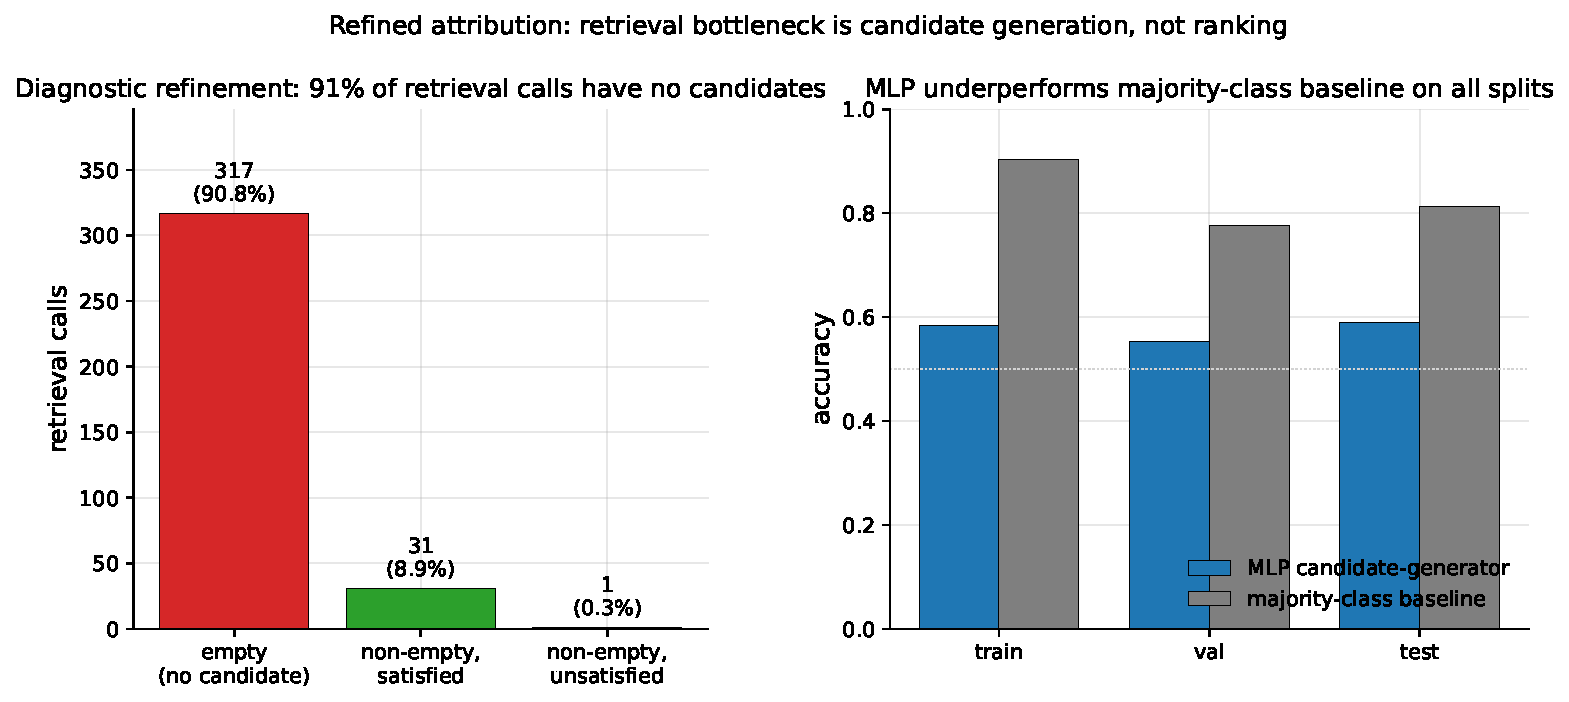
\includegraphics[width=0.95\linewidth]{figures/fig_refined_attribution.pdf}
\caption{Refined attribution diagnostic. \emph{Left:} 349 retrieval calls aggregated across 10 seeds; 317 (90.8\%) returned empty candidate sets, 31 (8.9\%) returned at least one satisfied candidate, only 1 (0.3\%) returned candidates that were ranked but unsatisfied. The bottleneck is candidate generation, not candidate ranking. \emph{Right:} the trained MLP underperforms a majority-class baseline on all three seed-disjoint splits, confirming that instantaneous state features alone are insufficient to predict candidate eligibility.}
\label{fig:refined-attribution}
\end{figure}

The MLP underperforms majority-class on accuracy across all splits and
achieves only moderate precision at fixed recall. Instantaneous state
features are insufficient to predict candidate eligibility downstream. This is
the negative-but-informative finding referenced in \S\ref{sec:refined-attribution}:
the framework's ``retrieval-limited'' attribution refines to
``memory-accumulation-limited'' rather than ``ranking-limited''.

\subsection{CommNet-style learned communication baseline (\S\ref{sec:multi-agent-results})}

\textbf{Policy architecture.} Per-agent observation is 4-dim direction one-hot
$+$ $5\!\times\!5\!\times\!5$ local cell-type window (125) $+$ 2-dim normalised
position $=$ 131. Shared-weights encoder $131{\to}64{\to}64$ (ReLU), 16-dim
comm projection, peer mean-pool (excluding self), combine $80{\to}64$ (ReLU),
actor head $64\!\to\!4$ (TURN\_LEFT, TURN\_RIGHT, FORWARD, NOOP), critic head
$64\!\to\!1$. This is a CommNet-style learned-communication architecture~\citep{sukhbaatar2016commnet}.

\textbf{Training.} REINFORCE~\citep{williams1992simple} with value-baseline; loss $=\!-\,\mathrm{mean}(\log\pi(a)\cdot(R\!-\!V))\,+\,0.5\cdot\mathrm{MSE}(V,R)\,-\,0.01\cdot H[\pi]$; Adam $\text{lr}=3{\cdot}10^{-4}$, gradient clipping $1.0$. Reward shaping: $+1.0$ on first success per agent, $-0.01$ step cost, $-0.1$ per hazard contact. 2000 episodes cycling 200 environment seeds, wall-clock $100$\,s on CPU. Held-out eval: 50 environment seeds 250--299.

\textbf{Training curve.} Episode-level success (last-100 window) stays in
$[0.13, 0.23]$ throughout training; no monotonic improvement after $\sim\!200$
episodes. The policy converges to a local optimum where one of three agents
finds water by chance.

\begin{figure}[h]
\centering
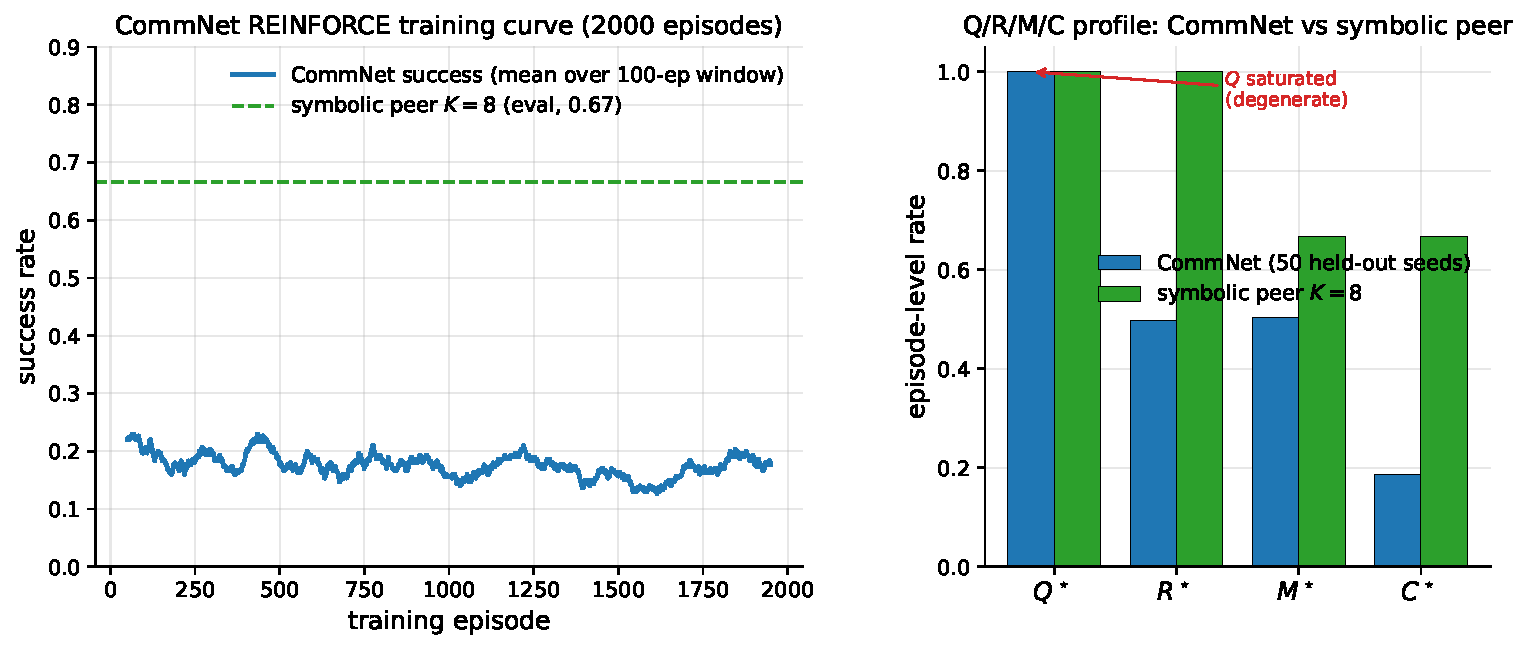
\includegraphics[width=0.95\linewidth]{figures/fig_commnet_baseline.pdf}
\caption{Learned-communication baseline diagnostics. \emph{Left:} CommNet training curve (smoothed success rate over a 100-episode window) over 2000 training episodes; success stays below 0.25 throughout. The dashed line is the symbolic peer architecture at $K\!=\!8$ on the same scenario for reference. \emph{Right:} Q/R/M/C profile of the trained CommNet on 50 held-out seeds vs symbolic peer at $K\!=\!8$. $Q^\star$ is saturated at $1.0$ on CommNet (degenerate by construction); $R/M$ collapse together; only on the symbolic architecture are the conditional rates separated.}
\label{fig:commnet}
\end{figure}

\textbf{Q/R/M/C evaluation (50 held-out seeds, stochastic action sampling).}

\begin{table}[h]
\centering
\small
\begin{tabular}{l c}
\toprule
Quantity & Value \\
\midrule
$Q^\star$ rate                              & \textbf{1.00} (saturated) \\
$R^\star$ rate                              & 0.50 \\
$M^\star$ rate                              & 0.50 (collapses onto $R$) \\
$C^\star$ rate                              & 0.19 \\
$P(R \mid Q)$                               & 0.50 \\
$P(M \mid R)$                               & 1.00 \\
$P(C \mid M)$                               & 0.42 \\
Success rate                                & 0.19 \\
Mean steps                                  & 80 (budget exhausted) \\
\bottomrule
\end{tabular}
\end{table}

Compare to the symbolic peer architecture at $K{=}8$: $P(M^\star|R^\star){=}0.69$, $P(C^\star|M^\star){=}0.87$, success $\sim 0.65$.

\paragraph{PPO variant: structural degeneracy verified at competitive success.}
A PPO-trained~\citep{schulman2017proximal} variant of the same CommNet architecture (clip $\epsilon{=}0.2$, generalized advantage estimation~\citep{schulman2016gae} with $\lambda{=}0.95$, $\gamma{=}0.99$, 4 PPO epochs per rollout, 64 rollouts per update, 200 updates, $\approx 96$ minutes on a single CPU core; full setup in \texttt{experiments/commnet\_ppo\_baseline/train\_ppo\_commnet.py}) reaches $0.667$ success on 100 held-out seeds --- competitive with the symbolic peer architecture at $K{=}8$ ($0.65$).

\begin{table}[h]
\centering
\small
\caption{REINFORCE vs PPO CommNet vs symbolic peer ($K{=}8$) on the scarcity scenario ($N{=}3$, $T{=}2$, asymmetric, hazard $0.05$). PPO is competitive on success rate, yet still exhibits Q-saturation and R/M collapse --- the diagnostic claim verified, not asserted.}
\label{tab:ppo-commnet}
\begin{tabular}{l c c c}
\toprule
Metric & CommNet REINFORCE & \textbf{CommNet PPO} & Symbolic peer ($K{=}8$) \\
\midrule
Success rate                  & 0.19   & \textbf{0.667} & 0.65 \\
$Q^\star$ rate                & 1.00   & \textbf{1.00}  & 0.99 \\
$R^\star$ rate                & 0.50   & \textbf{0.997} & 0.69 \\
$M^\star$ rate                & 0.50   & \textbf{0.997} & 0.69 \\
$P(M^\star|R^\star)$          & 1.00   & \textbf{1.00}  & 0.69 \\
$P(C^\star|M^\star)$          & 0.42   & \textbf{0.67}  & 0.87 \\
R/M separated?                & no     & \textbf{no}    & \textbf{yes} \\
\bottomrule
\end{tabular}
\end{table}

The PPO result converts the structural argument from an assertion (``training budget would not change this'') to a measurement: $Q^\star$ remains saturated at 1.00, $P(M^\star|R^\star)$ remains 1.00 (R/M collapse), even at competitive success. The Q stage is degenerate by construction in any policy whose communication channel is a real-valued vector with a learned linear projection --- the channel is never informatively empty, regardless of training budget --- and without an explicit symbolic target-lock interface the M event cannot separate from R. Only architectures with an explicit \emph{query/lock} interface (the symbolic stack of \S\ref{sec:archs}) expose stage-separable Q/R/M/C events.

\section{Reproducibility commands}
\label{app:repro}

An anonymized public repository accompanies this submission. The main paper artifacts were generated from the following scripts; \texttt{PYTHONPATH=.} and a Python 3 virtual environment with \texttt{numpy}, \texttt{scipy}, \texttt{pandas}, \texttt{matplotlib}, \texttt{imageio}, \texttt{gymnasium}, and \texttt{minigrid} are assumed throughout.

\subsection*{One-command reproduction (multi-agent block, $\approx 22$ minutes on 8 cores)}
\path{bash scripts/reproduce_paper.sh}

\subsection*{Clean Paper 1 suite}
\begin{itemize}[leftmargin=16pt]
\item smoke suite (all local non-LLM blocks): \path{python scripts/run_paper1_clean_experiments.py --mode smoke --skip_llm --out_dir tmp/paper1_clean_experiments_smoke}
\item full local suite (single-agent, oracle, multi-agent, CommNet, portability/noise): \path{python scripts/run_paper1_clean_experiments.py --mode full --skip_llm --workers 8 --out_dir tmp/paper1_clean_experiments_full}
\item LLM TextNav step-budget sweep (requires local Ollama), run once per budget $K'\in\{6,12,25\}$: \path{python -m experiments.llm_collective.run_model_sweep --models qwen3:4b llama3.1:latest --episodes 8 --step_limit <K'> --out_dir tmp/llm_steplimit_<K'>}
\end{itemize}

\subsection*{Single-agent (\S\ref{sec:validation}--\S\ref{sec:oracle})}
\begin{itemize}[leftmargin=16pt]
\item article benchmark and learned-baseline suite: \path{scripts/benchmark_symbolic_memory_article.py}
\item article analysis and figure generation: \path{scripts/analyze_symbolic_memory_article.py}
\item synthetic factorization sanity check: \path{scripts/validate_qrmc_factorization.py}
\item oracle-stage intervention benchmark: \path{scripts/benchmark_oracle_stage_interventions.py}
\item BabyAI transfer benchmark: \path{scripts/compare_semnav_babyai.py}
\end{itemize}

\subsection*{Multi-agent (\S\ref{sec:multi-agent-results})}
\begin{itemize}[leftmargin=16pt]
\item Base batch --- peer at $K\in\{1,2,4,8,16\}$ \emph{and} the three cadence-free architectures (independent, shared bus, central aggregator), 40 seeds ($25{,}920$ runs $=16{,}200$ peer $+\,9{,}720$ cadence-free), $\approx 18$ min:
\path{python experiments/big_experiment/exp_cadence_phase.py --mode full --workers 8 --out_dir tmp/big_experiment_qrmc_40}
\item Extended-cadence batch --- peer at $K\in\{32,48,64\}$ only ($9{,}720$ runs), $\approx 4$ min:
\path{python experiments/big_experiment/exp_extra_K.py --workers 8 --out_dir tmp/big_experiment_extraK}
\item[] \emph{Note.} These two batches partition the $35{,}640$ total by \emph{cadence range}; the architecture-wise partition of Appendix~\ref{app:design} ($25{,}920$ peer over all eight cadences vs.\ $9{,}720$ cadence-free) reuses the same two totals for \emph{different} subsets (a coincidence of $3$ extended cadences $\times\,3{,}240 = 3$ cadence-free architectures $\times\,3{,}240$). The combined log is \path{tmp/paper1_clean_experiments_full/multiagent_cadence_full/runs.csv}.
\item Q/R/M/C stage analysis and bootstrap CIs:
\path{python experiments/big_experiment/analyze_qrmc.py --runs_csv tmp/big_experiment_qrmc_40/runs.csv --out_dir tmp/big_experiment_qrmc_40}
\item Multi-agent oracle interventions:
\path{python experiments/big_experiment/exp_oracle_interventions.py --workers 8 --out_dir tmp/big_experiment_oracle}
\item Phase 1--4 smoke tests:
\path{python scripts/run_all_smokes.py --out_dir tmp/all_smokes}
\item PPO-trained CommNet baseline (Table~\ref{tab:ppo-commnet}, $\approx 96$ min on a single CPU core):
\path{python -m experiments.commnet_ppo_baseline.train_ppo_commnet --total_updates 200 --rollouts_per_update 64}
\item Q/R/M/C eval of the PPO policy on 100 held-out seeds:
\path{python experiments/commnet_baseline/eval_with_qrmc.py --policy_path experiments/commnet_ppo_baseline/ppo_policy.pt --out_dir experiments/commnet_ppo_baseline --n_episodes 100}
\item MiniGrid-substrate portability sweep (\S\ref{sec:limitations}, 100 runs, $\approx 2$ min):
\path{python -m experiments.minigrid_multiagent_wrapper.run_portability_sweep --out_dir tmp/minigrid_portability}
\end{itemize}

\section{Asset and license note}
\label{app:assets}

The experiments use MiniGrid~\citep{MinigridMiniworld23} and BabyAI~\citep{chevalier2018babyai}, both released under the MIT License. The locally implemented baselines and benchmark runner scripts introduced in this paper will be released under the MIT License as part of the camera-ready artifact package.

\clearpage
\FloatBarrier
\input{checklist.tex}

\end{document}
